\documentclass{cmspaper}
\usepackage{graphicx}
\usepackage{amsmath}
\usepackage{amssymb}
\usepackage{subfigure}
\usepackage{multirow}
\usepackage[pdfborder=0 0 0,
            colorlinks,
            urlcolor = blue,
            linkcolor = black,
            citecolor = black,
            menucolor = black,]
           {hyperref}
%% \usepackage[colorlinks]{hyperref}
%% \usepackage{url}
\usepackage[toc,page]{appendix}
\renewcommand{\appendixname}{Appendix}
%% \renewcommand{\appendixtocname}{List of appendices}

% % useful definitions

% processes
\def\dyee {\ensuremath{Z/\gamma^*\to ee}}
\def\dymm {\ensuremath{Z/\gamma^*\to\mu\mu}}
\def\dytt {\ensuremath{Z/\gamma^*\to\tau\tau}}
\def\zee {\ensuremath{Z\to ee}}
\def\zmm {\ensuremath{Z\to\mu\mu}}
\def\ztt {\ensuremath{Z\to\tau\tau}}
\def\ttbar {\ensuremath{t\bar{t}}}
\def\wwll {\ensuremath{WW\to l^+l^-}}
\def\wwlulu{\ensuremath{WW\to l^+\nu l^-\bar{\nu}}}
\def\ww {\ensuremath{WW}}
\def\hww {\ensuremath{H\to WW}}
\def\wz{\ensuremath{WZ}}
\def\zz{\ensuremath{ZZ}}
\def\wgamma{\ensuremath{W\gamma}}
\def\wjets{\ensuremath{W+}jets} 
\def\tw{\ensuremath{tW}} 
\def\singletopt{\ensuremath{t} ($t$-chan)} 
\def\singletops{\ensuremath{t} ($s$-chan)} 
\def\all{all}
\def\ee{\ensuremath{ee}}
\def\emu{\ensuremath{e\mu}}
\def\mm{\ensuremath{\mu\mu}}

%units
\newcommand{\TeV}{\ensuremath{\mathrm{Te\kern -0.1em V}}}
\newcommand{\GeV}{\ensuremath{\mathrm{Ge\kern -0.1em V}}}

%others
\def\pt{\ensuremath{p_T}}
\def\ipb{pb\ensuremath{^{-1}}}
\def\ifb{fb\ensuremath{^{-1}}}
\def\et{\ensuremath{E_T}}
\def\met{\ensuremath{E\!\!\!\!/_T}}
\def\fBrem{\ensuremath{f_{\rm brem}}}
\def\pin{\ensuremath{p_{\rm in}}}
\def\pout{\ensuremath{p_{\rm out}}}

\newcommand{\CLs}{\ensuremath{CL_\mathrm{s}}}
\newcommand{\CLb}{\ensuremath{CL_\mathrm{b}}}
\newcommand{\CLsb}{\ensuremath{CL_\mathrm{s+b}}}

\newcommand{\GeV}{\ensuremath{\mathrm{Ge\kern -0.1em V}}}
\newcommand{\TeV}{\ensuremath{\mathrm{Te\kern -0.1em V}}}
\newcommand{\TeVcc}{\ensuremath{\,\mathrm{Te\kern -0.1em V\!/c}^2}}
\newcommand{\GeVcc}{\ensuremath{\,\mathrm{Ge\kern -0.1em V\!/c}^2}}
\newcommand{\MeVcc}{\ensuremath{\,\mathrm{Me\kern -0.1em V\!/c}^2}}
\newcommand{\GeVc}{\ensuremath{\mathrm{Ge\kern -0.1em V}\!/c}}
\newcommand{\nanob}{\mbox{{\rm ~nb}~}}
\newcommand{\fb}{\ensuremath{\mathrm{fb}}}
\newcommand{\pb}{\ensuremath{\mathrm{pb}}}
\newcommand{\ifb}{\ensuremath{\mathrm{fb^{-1}}}}
\newcommand{\ipb}{\ensuremath{\mathrm{pb^{-1}}}}
\newcommand{\grad}{\ensuremath{^{\circ}}}
%
% Special user made math symbols
%
\newcommand{\lsim}{\raisebox{-1.5mm}{$\:\stackrel{\textstyle{<}}{\textstyle{\sim}}\:$}}
\newcommand{\gsim}{\raisebox{-1.5mm}{$\:\stackrel{\textstyle{>}}{\textstyle{\sim}}\:$}}

% particles

\newcommand{\pipm}{\ensuremath{\pi^{\pm}}}
\newcommand{\pizero}{\ensuremath{\pi^{0}}}
\newcommand{\Hi}{\ensuremath{\mathrm{H}}}
\newcommand{\W}{\ensuremath{\mathrm{W}}}
\newcommand{\Wjets}{\ensuremath{\mathrm{W+jets}}}
\newcommand{\Zjets}{\ensuremath{\mathrm{Z+jets}}}
\newcommand{\Wt}{\ensuremath{\mathrm{Wt}}}
\newcommand{\Wstar}{\ensuremath{\mathrm{W}^{*}}}
\newcommand{\Wparenthesisstar}{\ensuremath{\mathrm{W}^{(*)}}}
\newcommand{\WW}{\ensuremath{\W^+\W^-}}
\newcommand{\Z}{\ensuremath{\mathrm{Z}}}
\newcommand{\Zstar}{\ensuremath{\mathrm{Z}^{*}}}
\newcommand{\Astar}{\ensuremath{\mathrm{\gamma}^{*}}}
\newcommand{\ZZ}{\ensuremath{\Z\Z}}
\newcommand{\WZ}{\ensuremath{\W\Z}}
\newcommand{\Wgstar}{\ensuremath{\W\Astar}}
\newcommand{\E}{\ensuremath{\mathrm{e}}}
\newcommand{\Ep}{\ensuremath{\mathrm{e}^{+}}}
\newcommand{\Em}{\ensuremath{\mathrm{e}^{-}}}
\newcommand{\Epm}{\ensuremath{\mathrm{e}^{\pm}}}
\newcommand{\Emp}{\ensuremath{\mathrm{e}^{\mp}}}
\newcommand{\M}{\ensuremath{\mu}}
\newcommand{\Mp}{\ensuremath{\mu^{+}}}
\newcommand{\Mm}{\ensuremath{\mu^{-}}}
\newcommand{\Mpm}{\ensuremath{\mu^{\pm}}}
\newcommand{\Mmp}{\ensuremath{\mu^{\mp}}}
\newcommand{\Tau}{\ensuremath{\tau}}
\newcommand{\Nu}{\ensuremath{\nu}}
\newcommand{\Nubar}{\ensuremath{\bar{\nu}}}
\newcommand{\Lep}{\ensuremath{\ell}}
\newcommand{\Lepp}{\ensuremath{\ell^{+}}}
\newcommand{\Lepm}{\ensuremath{\ell^{-}}}
\newcommand{\Lprime}{\ensuremath{\Lep^{\prime}}}
\newcommand{\Prot}{\ensuremath{\mathrm{p}}}
\newcommand{\Pbar}{\ensuremath{\bar{\mathrm{p}}}}
\newcommand{\PP}{\Prot\Prot}
\newcommand{\PPbar}{\Prot\Pbar}
\newcommand{\ttbar}{\ensuremath{\mathrm{t}\bar{\mathrm{t}}}}
\newcommand{\qq}{\ensuremath{\mathrm{q}\mathrm{q}}}
%\newcommand{\bbbar}{\ensuremath{\mathrm{b}\bar{\mathrm{b}}}}
\newcommand{\Wtb}{\ensuremath{\W\mathrm{t}\mathrm{b}}}
\newcommand{\Top}{\ensuremath{\mathrm{t}}}
\newcommand{\Bot}{\ensuremath{\mathrm{b}}}
\newcommand{\Atop}{\ensuremath{\bar{\mathrm{t}}}}
\newcommand{\Abot}{\ensuremath{\bar{\mathrm{b}}}}
% arrow
\newcommand{\To}{\ensuremath{\rightarrow}}

% masses
\newcommand{\mHi}{\ensuremath{m_{\mathrm{H}}}}
\newcommand{\mW}{\ensuremath{m_{\mathrm{W}}}}
\newcommand{\mZ}{\ensuremath{m_{\mathrm{Z}}}}
\newcommand{\mll}{\ensuremath{m_{\Lep\Lep}}}
\newcommand{\mt}{\ensuremath{m_{\mathrm{T}}}}

% kinematics
\newcommand{\pt}{\ensuremath{p_\mathrm{T}}}
\newcommand{\ptveto}{\ensuremath{\pt^\mathrm{veto}}}
\newcommand{\ptl}{\ensuremath{p_\perp^{\Lep}}}
\newcommand{\ptlmax}{\ensuremath{p_{\mathrm{T}}^{\Lep,\mathrm{max}}}}
\newcommand{\ptlmin}{\ensuremath{p_{\mathrm{T}}^{\Lep,\mathrm{min}}}}
\newcommand{\met}{\ensuremath{\Et^{\mathrm{miss}}}}
\newcommand{\delphill}{\ensuremath{\Delta\phi_{\Lep\Lep}}}
\newcommand{\deletall}{\ensuremath{\Delta\eta_{\Lep\Lep}}}
\newcommand{\delphimetl}{\ensuremath{\Delta\phi_{\met\Lep}}}
\newcommand{\Et}{\ensuremath{E_\mathrm{T}}}
\newcommand{\delR}{\ensuremath{\Delta R}}
\newcommand{\Eta}{\ensuremath{\eta}}

%efficiencies
\newcommand{\effsig}{\ensuremath{\varepsilon_{\mathrm{bkg}}^{\mathrm{S}}}}
\newcommand{\effnorm}{\ensuremath{\varepsilon_{\mathrm{bkg}}^{\mathrm{N}}}}
\newcommand{\Nsig}{\ensuremath{N_{\mathrm{bkg}}^{\mathrm{S}}}}
\newcommand{\Nnorm}{\ensuremath{N_{\mathrm{bkg}}^{\mathrm{N}}}}

% processes
\newcommand{\dyee}{\ensuremath{Z/\gamma^*\to ee}}
\newcommand{\dymm}{\ensuremath{Z/\gamma^*\to\mu\mu}}
\newcommand{\dytt}{\ensuremath{Z/\gamma^*\to\tau\tau}}
\newcommand{\dyll}{\ensuremath{Z/\gamma^*\to\ell\ell}}
\newcommand{\dy}{\ensuremath{Z/\gamma^*}}
\newcommand{\zee}{\ensuremath{Z\to ee}}
\newcommand{\zmm}{\ensuremath{Z\to\mu\mu}}
\newcommand{\ztt}{\ensuremath{Z\to\tau\tau}}
%\newcommand{\ttbar}{\ensuremath{t\bar{t}}}
\newcommand{\ppww}{\ensuremath{pp \to W^+W^-}}
\newcommand{\wwll}{\ensuremath{WW\to \ell^+\ell^-}}
\newcommand{\wwlnln}{\ensuremath{W^+W^-\to \ell^+\nu \ell^-\bar{\nu}}}
\newcommand{\ww}{\ensuremath{WW}}
\newcommand{\wwpm}{\ensuremath{W^+W^-}}
\newcommand{\hww}{\ensuremath{H\to W^+W^-}}
\newcommand{\wz}{\ensuremath{WZ}}
\newcommand{\zz}{\ensuremath{ZZ}}
\newcommand{\wgamma}{\ensuremath{W\gamma}}
\newcommand{\wjets}{\ensuremath{W+}jets} 
\newcommand{\tw}{\ensuremath{tW}} 
\newcommand{\singletopt}{\ensuremath{t} ($t$-chan)} 
\newcommand{\singletops}{\ensuremath{t} ($s$-chan)} 
\newcommand{\zx}{\ensuremath{\mathrm{DY/WZ/ZZ}}}
\newcommand{\zv}{\ensuremath{\mathrm{WZ/ZZ}}}
\newcommand{\z}{\ensuremath{\mathrm{Z}}}
\newcommand{\routin}{\ensuremath{R_{out/in}}}

%other 
\def\fixme{({\bf FixMe})}
\newcommand{\ee}{\ensuremath{ee}}
\newcommand{\emu}{\ensuremath{e\mu}}
\def\mm{\ensuremath{\mu\mu}}

% integrated luminosity
\newcommand{\intlumiSevenTeV}{4.92~\ifb}
\newcommand{\intlumiEightTeV}{1.62~\ifb}

%%%%%%%%%%%
%
\newcounter{myfootertablecounter}

\newcommand\myfootnotemark{%
  %\refstepcounter{footnote}%
  \addtocounter{footnote}{1}%
  \footnotemark[\thefootnote]%
}%

\newcommand\myfootnotetext[1]{%
  \addtocounter{myfootertablecounter}{1}
  \footnotetext[\value{myfootertablecounter}]{#1}
}

% from now on, myfootnote has to be used rather than footnote to
% adapt the myfootercounter
\newcommand\myfootnote[1]{%
  \addtocounter{myfootertablecounter}{1}
  \footnote{#1}
}%



\setcounter{topnumber}{1}
\setcounter{bottomnumber}{1}

%===================================================================================================
\begin{document}
\begin{titlepage}

  \analysisnote{2011/*}

  \date{\today}

  \title{A Higgs Boson Search in the Fully Leptonic $W^+W^-$ Final State - Update for Lepton-Photon 2011}

  \begin{Authlist}
%
L.~Bauerdick, K.~Burkett, I.~Fisk, Y.~Gao, O.~Gutsche, B.~Hooberman, S.~Jindariani, S.~Tkaczyk, V. Martinez Outschoorn, 
\Instfoot{fnal}{Fermilab National Accelerator Laboratory, Batavia, USA}
%
G.~Bauer, J.~Bendavid, E.~Butz, M.~Chan, V.~Dutta, G.~G\'omez-Ceballos, M.~Goncharov, K.~Hahn, P.~Harris, M.~Klute, S.~Nahn, C.~Paus, D.~Ralph, F.~Stoeckli, K.~Sumorok, K.~Sung, R.~Wolf, S.~Xie, M.~Yang, M.~Zanetti
\Instfoot{mit}{Laboratory for Nuclear Science, Massachusetts Institute of Technology, Cambridge, USA}
%
D.~Barge, C.~Campagnari, D.~Kovalskyi, V.~Krutelyov
\Instfoot{ucsb}{University of California, Santa Barbara, Santa Barbara, USA}
%
W.~Andrews, G.~Cerati, D.~Evans, F.~Golf, I.~MacNeill, S.~Padhi, Y.~Tu, F.~W\"urthwein, A.~Yagil, J.~Yoo
\Instfoot{ucsd}{University of California, San Diego, San Diego, USA}
%
I.~Kravchenko
\Instfoot{unl}{University of Nebraska-Lincoln, USA}

\end{Authlist}


  \begin{abstract}
  \end{abstract} 

\end{titlepage}
\tableofcontents
%\listoftables
%\listoffigures
\newpage 

%===================================================================================================
\appendix
  \section{Lepton-Photon Reload}
     \label{app:lp_reload}
     \subsection{Introduction}
     
This appendix describes the ``reload'' of the analysis described in the body
of this document for the Lepton Photon 2011 conference.
The reload primarily adds extra data to the existing analysis, but also 
includes minor technical changes described in this appendix.
We define the following naming conventions for the analyses described:

\begin{itemize}
    \item The EPS analysis refers to the methods and results documented in the body of this note.
    \item The LP analysis refers to the application of the EPS analysis methods to the extended dataset.
\end{itemize}

We define the following naming conventions for the datasets used:

\begin{itemize}
    \item The EPS dataset refers to the initial $\sim$ \intlumi~dataset described in Section \ref{sec:datasets}.
    \item The post-EPS dataset refers to the $\sim$ 0.5 fb$^{-1}$ dataset recorded after the EPS2011 conference.
    \begin{itemize}
        \item August 5th ReReco $XXX<run<YYY$.
        \item PromptReco V6 $AAA<run<BBB$.
    \end{itemize}
    \item The LP dataset refers to the total $\sim$ \lpintlumi~dataset.
\end{itemize}

We performed this reload according to the following methodology:

\begin{itemize}
    \item We first identified a number of necessary technical changes to the analysis.  
These are summarised in Section \ref{app:lp_technical_changes}.
    \item We then validated these changes by performing a side by side comparison of 
the analysis on the EPS dataset with and without these changes.
These are summarised in Section \ref{sec:lpreload_technical_validation}.
Having convinced ourselves that the analysis was understood, we proceeded to add more data.
    \item We first validated the post-EPS dataset against the existing results for the EPS dataset.
We found good agreement in the background estimates and data to simulation scale factors.
    \item We then performed the background estimations and full analysis on the LP dataset.
The results of the reloaded analysis are described in Section \ref{sec:lpreload_results}.
\end{itemize}


     \subsection{Definition of Reload}
    \label{app:lp_technical_changes}
     
Since the EPS analysis was completed, we identified the following small technical
changes required to make the analysis more consistent:

\begin{itemize}
    \item The integrated luminosity estimate for EPS dataset is revised from 1.092 fb$^{-1}$ to 1.143 fb$^{-1}$.
    \item The \dytt and \dyll backgrounds are considered separately.
    \item The data to simulation scale factors for pile-up, lepton and trigger efficiencies are 
always applied to the simulation both when deriving and applying scale factors for background estimation.
    \item The residual jet energy corrections are included.
\end{itemize}

We additionally considered the effect on the analysis of adding FIXME describe MT cut here.
The effect of these changes is evaluated on the EPS dataset in Section \ref{sec:lp_technical_validation}.



     \subsection{Post-EPS Data Validation}
     \label{app:lp_validation}
     \subsubsection{Lepton and Trigger Efficiency}
     This is a Lepton and Trigger Efficiency

     \subsubsection{PU reweighting}
     This is a PU reweighting

    \subsubsection{Summary of Data Validation}
    
We find the post-EPS data to be consistent with the EPS data with regard to trigger and
lepton efficiencies. We find good agreement between data and MC for the distribution of the number
of reconstructed vertices per event after re-weighting based on the expected number of pile-up events.
We inspected the relevant kinematic variables (see Section \ref{app:lp_postEPSdist} for details) and find no significant
discrepancies between the two data samples.



     \subsection{Background Estimation for \lpintlumi}
    \label{app:lp_bkgestim}
     This is a background Estimation for 1.545$\fb$


     \subsection{Final limits for \lpintlumi}
    \label{app:lp_limits}
     This is a final limit


     \subsection{Conclusions}
     This is a conclusion


    \subsection{Data Validation}
    \label{app:lp_postEPSdist}
    Plots are normalized to 1$/fb$. 
Error bars are the sum in quadrature of the statistical uncertainty of EPS and post-EPS data. 
EPS dataset corresponds to run$<$170826, post-EPS to run$\geq$170826.

\clearpage

\begin{figure}[!hbtp]
\centering
\subfigure[]{
\centering
\label{subfig:lp_dPhi_ww0j}
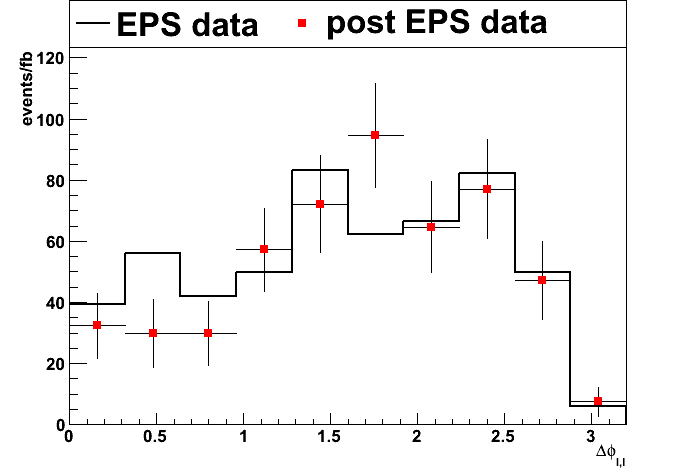
\includegraphics[width=.32\textwidth]{lp_figures/postEPSvalid/hm0/dPhi_ww0j.png}}
\subfigure[]{
\centering
\label{subfig:lp_dilepmass_ww0j}
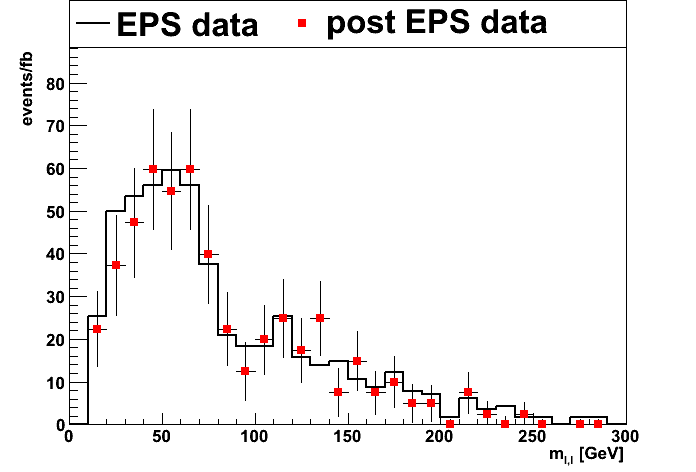
\includegraphics[width=.32\textwidth]{lp_figures/postEPSvalid/hm0/dilepmass_ww0j.png}}\\
\subfigure[]{
\centering
\label{subfig:lp_dileppt_ww0j}
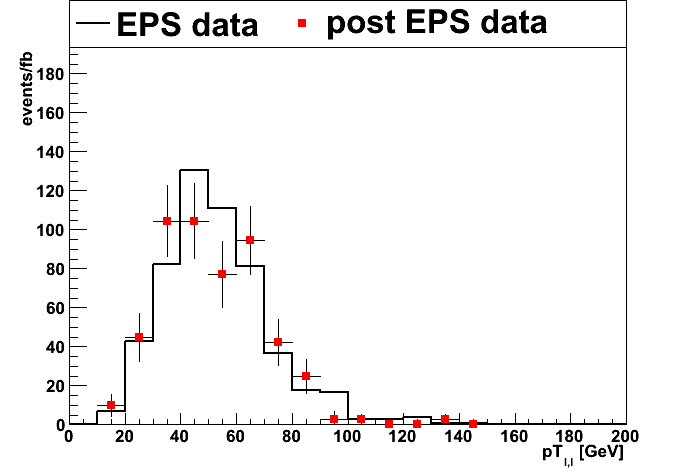
\includegraphics[width=.32\textwidth]{lp_figures/postEPSvalid/hm0/dileppt_ww0j.png}}
\subfigure[]{
\centering
\label{subfig:lp_type_ww0j}
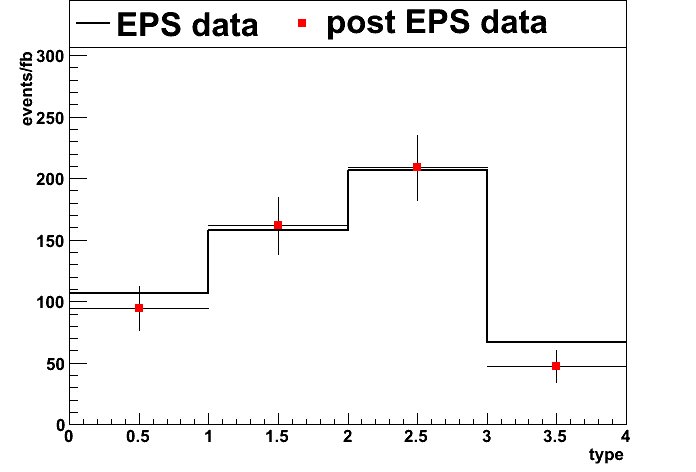
\includegraphics[width=.32\textwidth]{lp_figures/postEPSvalid/hm0/type_ww0j.png}}
\caption{EPS and post-EPS data comparison: 0-jet bin, all final states. 
\subref{subfig:lp_dPhi_ww0j} $\Delta\phi$ between the two leptons;
\subref{subfig:lp_dilepmass_ww0j} di-lepton invariant mass;
\subref{subfig:lp_dileppt_ww0j} di-lepton transverse momentum;
\subref{subfig:lp_type_ww0j} di-lepton type ($\mu\mu$=0, $\mu e$=2, $e\mu$=2, $ee$=3).
}
\label{fig:lp_ww0j_dilep}
\end{figure}

\begin{figure}[!hbtp]
\centering
\subfigure[]{
\centering
\label{subfig:lp_lep1pt_ww0j}
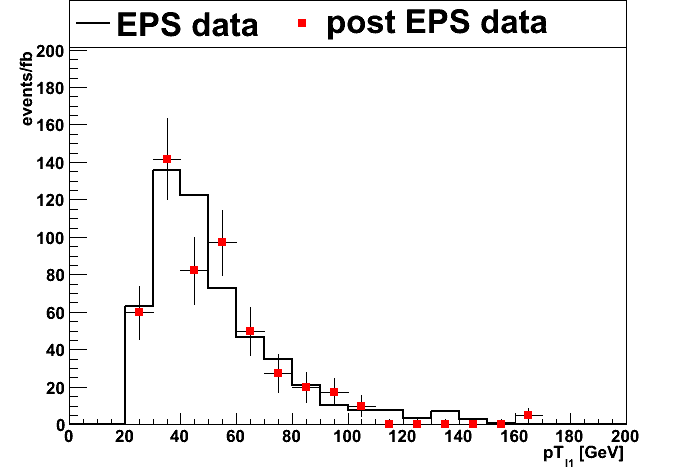
\includegraphics[width=.32\textwidth]{lp_figures/postEPSvalid/hm0/lep1pt_ww0j.png}}
\subfigure[]{
\centering
\label{subfig:lp_lep2pt_ww0j}
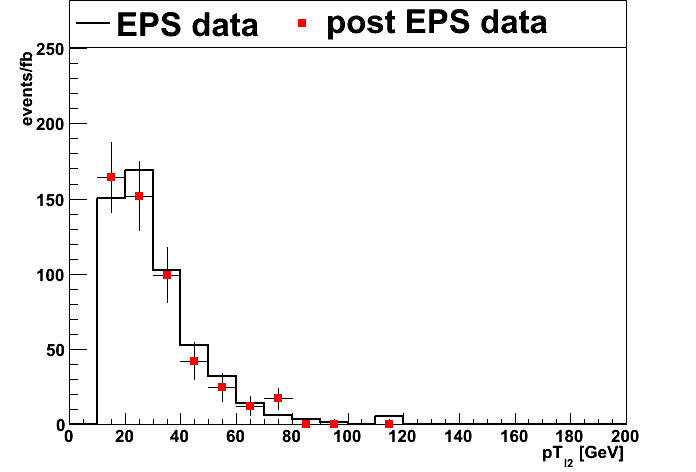
\includegraphics[width=.32\textwidth]{lp_figures/postEPSvalid/hm0/lep2pt_ww0j.png}}
\subfigure[]{
\centering
\label{subfig:lp_jet1pt_ww0j}
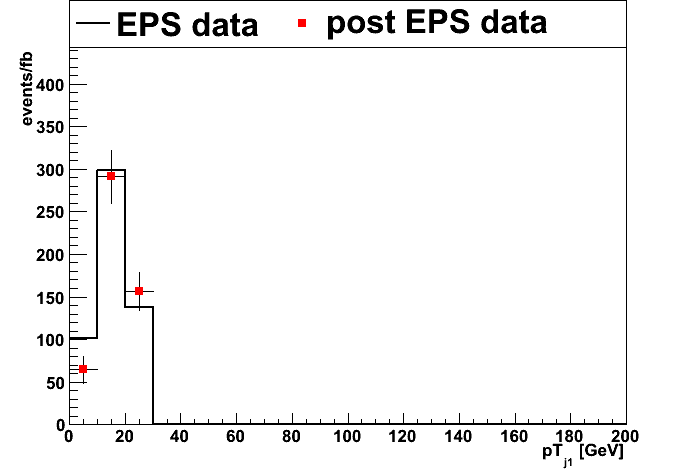
\includegraphics[width=.32\textwidth]{lp_figures/postEPSvalid/hm0/jet1pt_ww0j.png}}\\
\subfigure[]{
\centering
\label{subfig:lp_pmet_ww0j}
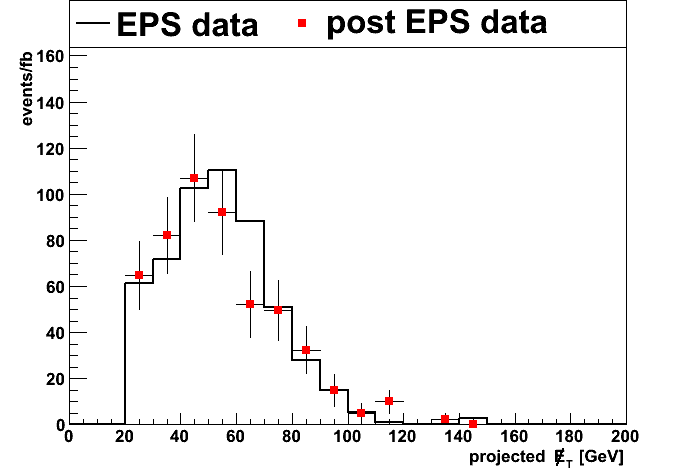
\includegraphics[width=.32\textwidth]{lp_figures/postEPSvalid/hm0/pmet_ww0j.png}}
\subfigure[]{
\centering
\label{subfig:lp_pTrackMet_ww0j}
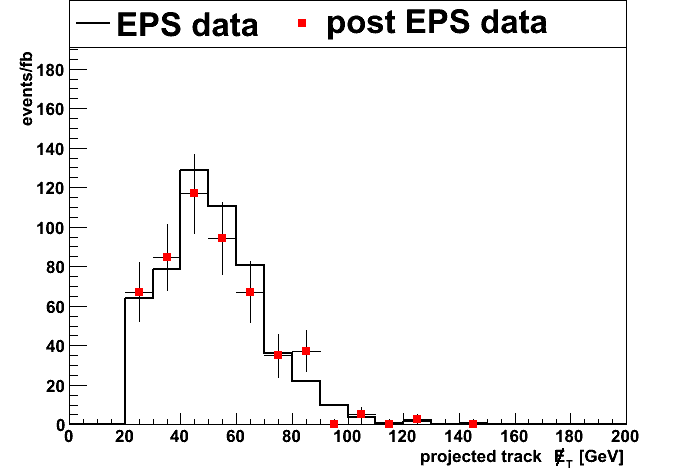
\includegraphics[width=.32\textwidth]{lp_figures/postEPSvalid/hm0/pTrackMet_ww0j.png}}
\subfigure[]{
\centering
\label{subfig:lp_mt_ww0j}
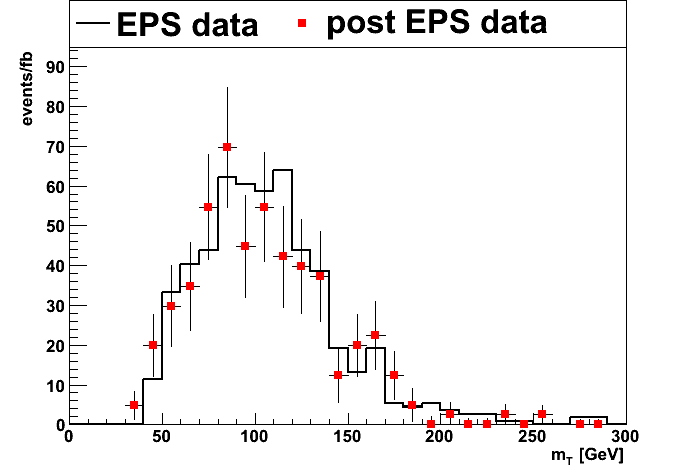
\includegraphics[width=.32\textwidth]{lp_figures/postEPSvalid/hm0/mt_ww0j.png}}
\caption{EPS and post-EPS data comparison: 0-jet bin, all final states. 
\subref{subfig:lp_lep1pt_ww0j} leading lepton $p_T$;
\subref{subfig:lp_lep2pt_ww0j} trailing lepton $p_T$;
\subref{subfig:lp_jet1pt_ww0j} leading jet $p_T$;
\subref{subfig:lp_pmet_ww0j} projected MET;
\subref{subfig:lp_pTrackMet_ww0j} projected track-MET;
\subref{subfig:lp_mt_ww0j} transverse mass of dilepton-MET system.
}
\label{fig:lp_ww0j_lepjetmet}
\end{figure}

\clearpage

\begin{figure}[!hbtp]
\centering
\subfigure[]{
\centering
\label{subfig:lp_dPhi_ww0jmm}
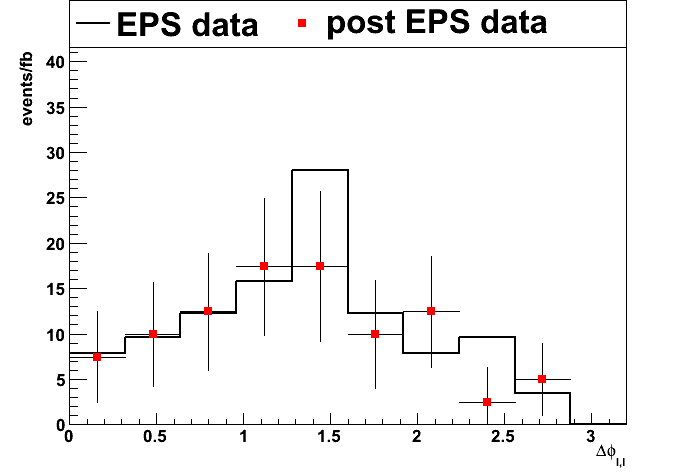
\includegraphics[width=.32\textwidth]{lp_figures/postEPSvalid/hm0/dPhi_ww0jmm.png}}
\subfigure[]{
\centering
\label{subfig:lp_dilepmass_ww0jmm}
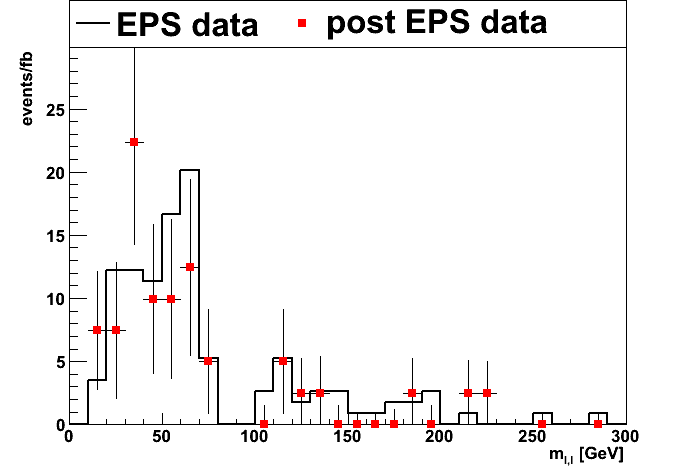
\includegraphics[width=.32\textwidth]{lp_figures/postEPSvalid/hm0/dilepmass_ww0jmm.png}}\\
\subfigure[]{
\centering
\label{subfig:lp_dileppt_ww0jmm}
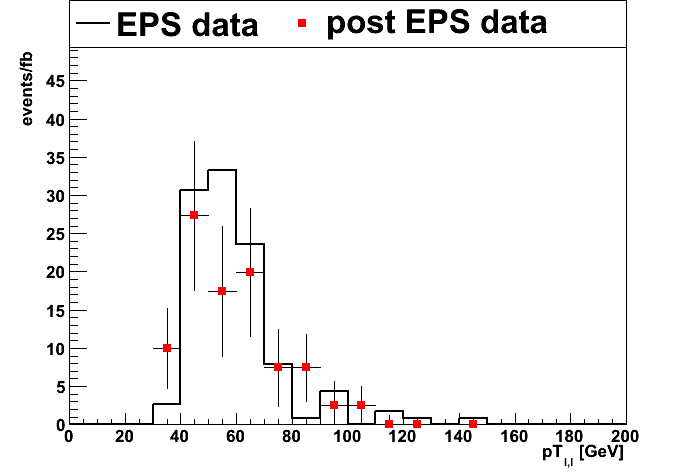
\includegraphics[width=.32\textwidth]{lp_figures/postEPSvalid/hm0/dileppt_ww0jmm.png}}
\subfigure[]{
\centering
\label{subfig:lp_type_ww0jmm}
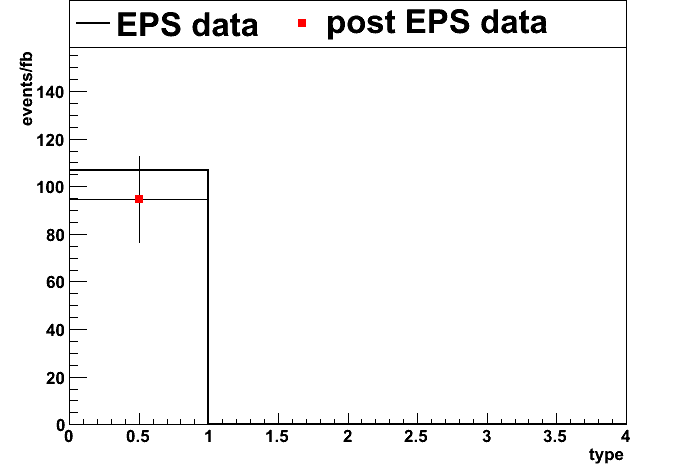
\includegraphics[width=.32\textwidth]{lp_figures/postEPSvalid/hm0/type_ww0jmm.png}}
\caption{EPS and post-EPS data comparison: 0-jet bin, $\mu\mu$ final state. 
\subref{subfig:lp_dPhi_ww0jmm} $\Delta\phi$ between the two leptons;
\subref{subfig:lp_dilepmass_ww0jmm} di-lepton invariant mass;
\subref{subfig:lp_dileppt_ww0jmm} di-lepton transverse momentum;
\subref{subfig:lp_type_ww0jmm} di-lepton type ($\mu\mu$=0, $\mu e$=2, $e\mu$=2, $ee$=3).
}
\label{fig:lp_ww0jmm_dilep}
\end{figure}

\begin{figure}[!hbtp]
\centering
\subfigure[]{
\centering
\label{subfig:lp_lep1pt_ww0jmm}
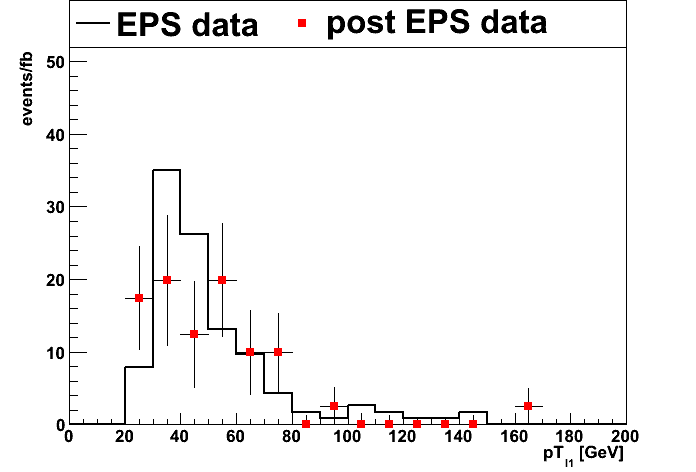
\includegraphics[width=.32\textwidth]{lp_figures/postEPSvalid/hm0/lep1pt_ww0jmm.png}}
\subfigure[]{
\centering
\label{subfig:lp_lep2pt_ww0jmm}
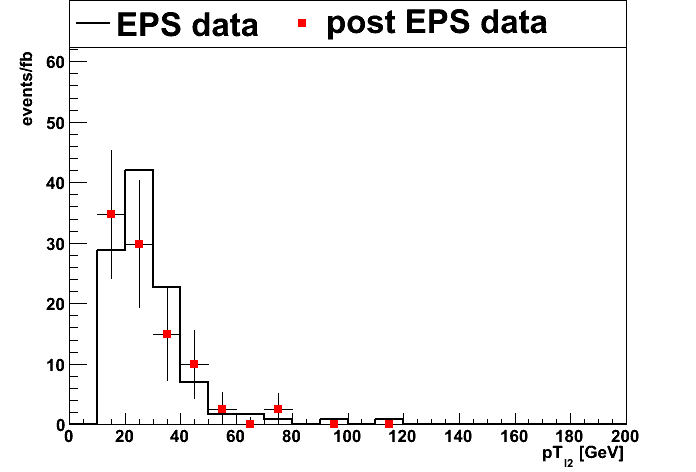
\includegraphics[width=.32\textwidth]{lp_figures/postEPSvalid/hm0/lep2pt_ww0jmm.png}}
\subfigure[]{
\centering
\label{subfig:lp_jet1pt_ww0jmm}
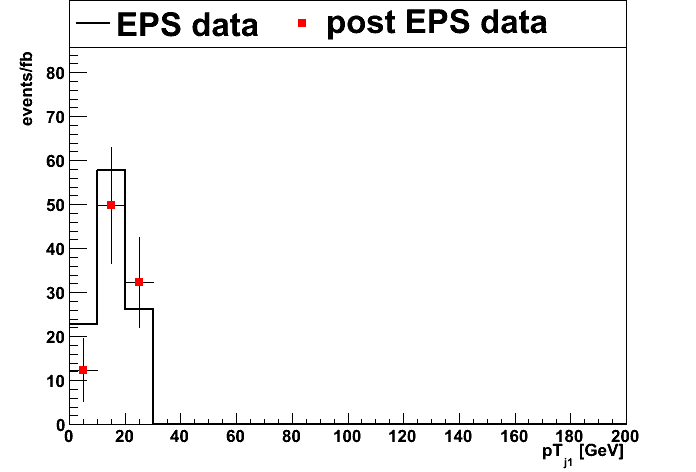
\includegraphics[width=.32\textwidth]{lp_figures/postEPSvalid/hm0/jet1pt_ww0jmm.png}}\\
\subfigure[]{
\centering
\label{subfig:lp_pmet_ww0jmm}
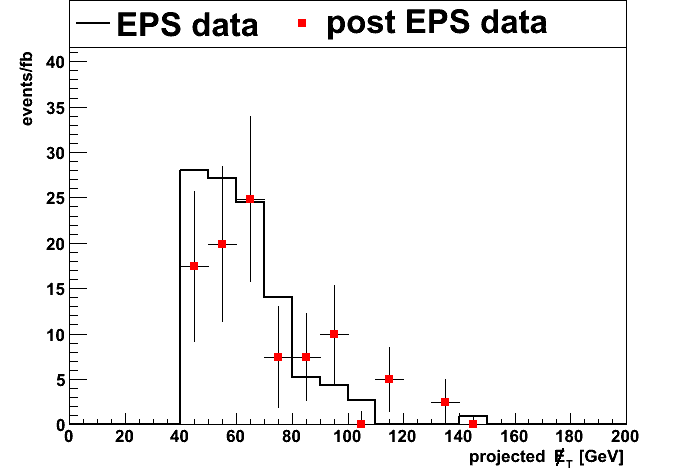
\includegraphics[width=.32\textwidth]{lp_figures/postEPSvalid/hm0/pmet_ww0jmm.png}}
\subfigure[]{
\centering
\label{subfig:lp_pTrackMet_ww0jmm}
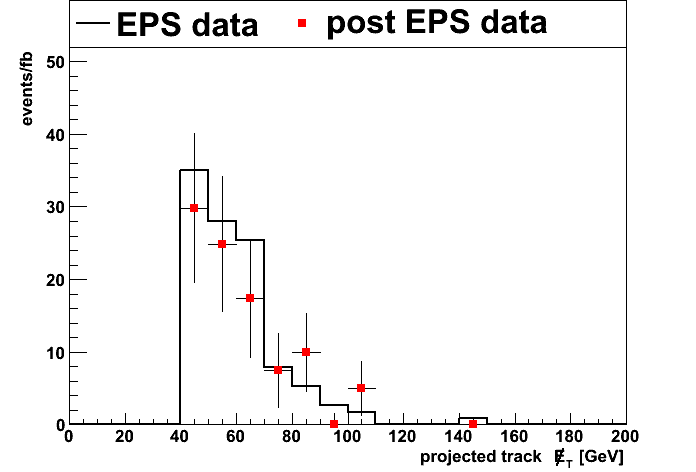
\includegraphics[width=.32\textwidth]{lp_figures/postEPSvalid/hm0/pTrackMet_ww0jmm.png}}
\subfigure[]{
\centering
\label{subfig:lp_mt_ww0jmm}
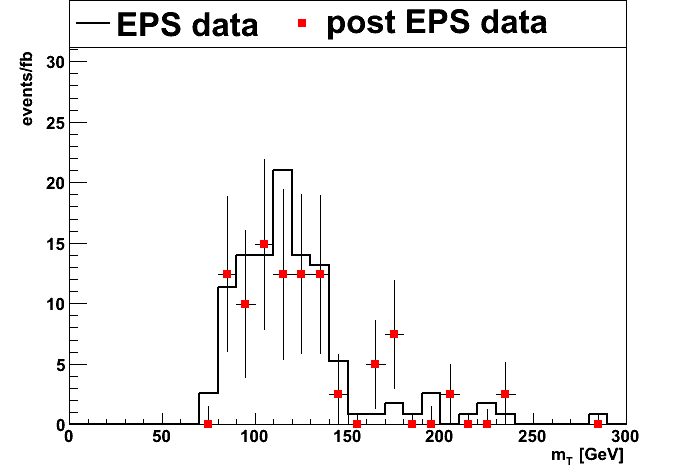
\includegraphics[width=.32\textwidth]{lp_figures/postEPSvalid/hm0/mt_ww0jmm.png}}
\caption{EPS and post-EPS data comparison: 0-jet bin, $\mu\mu$ final state. 
\subref{subfig:lp_lep1pt_ww0jmm} leading lepton $p_T$;
\subref{subfig:lp_lep2pt_ww0jmm} trailing lepton $p_T$;
\subref{subfig:lp_jet1pt_ww0jmm} leading jet $p_T$;
\subref{subfig:lp_pmet_ww0jmm} projected MET;
\subref{subfig:lp_pTrackMet_ww0jmm} projected track-MET;
\subref{subfig:lp_mt_ww0jmm} transverse mass of dilepton-MET system.
}
\label{fig:lp_ww0jmm_lepjetmet}
\end{figure}

\clearpage

\begin{figure}[!hbtp]
\centering
\subfigure[]{
\centering
\label{subfig:lp_dPhi_ww1j}
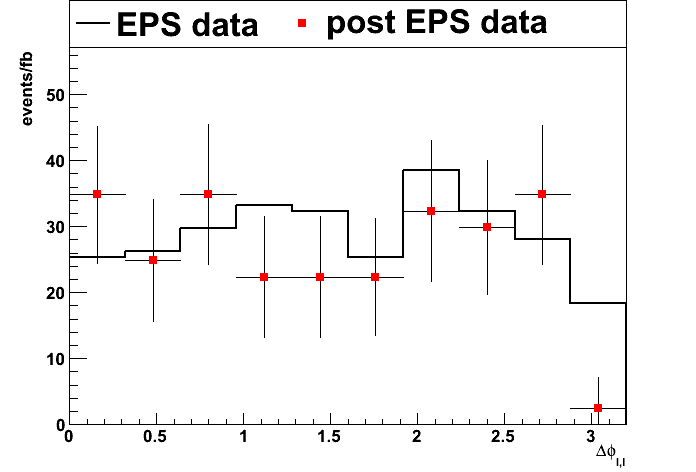
\includegraphics[width=.32\textwidth]{lp_figures/postEPSvalid/hm0/dPhi_ww1j.png}}
\subfigure[]{
\centering
\label{subfig:lp_dilepmass_ww1j}
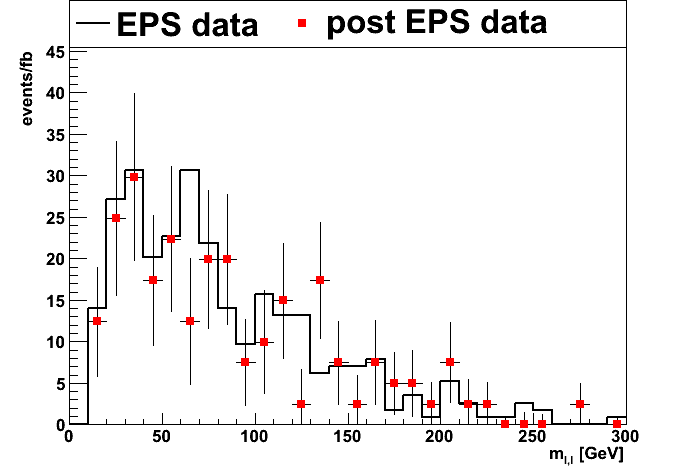
\includegraphics[width=.32\textwidth]{lp_figures/postEPSvalid/hm0/dilepmass_ww1j.png}}\\
\subfigure[]{
\centering
\label{subfig:lp_dileppt_ww1j}
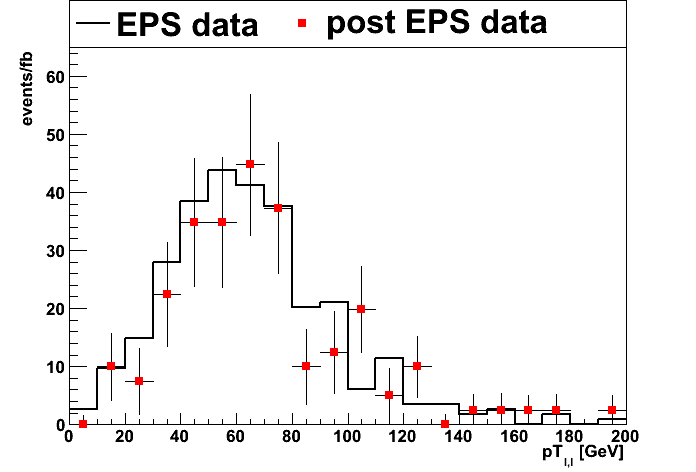
\includegraphics[width=.32\textwidth]{lp_figures/postEPSvalid/hm0/dileppt_ww1j.png}}
\subfigure[]{
\centering
\label{subfig:lp_type_ww1j}
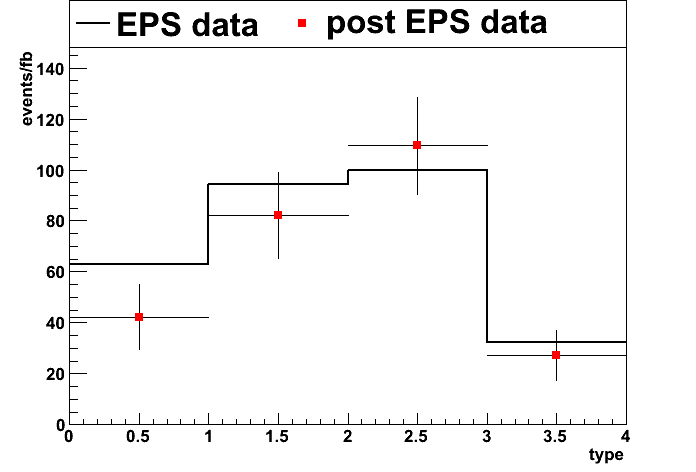
\includegraphics[width=.32\textwidth]{lp_figures/postEPSvalid/hm0/type_ww1j.png}}
\caption{EPS and post-EPS data comparison: 1-jet bin, all final states. 
\subref{subfig:lp_dPhi_ww1j} $\Delta\phi$ between the two leptons;
\subref{subfig:lp_dilepmass_ww1j} di-lepton invariant mass;
\subref{subfig:lp_dileppt_ww1j} di-lepton transverse momentum;
\subref{subfig:lp_type_ww1j} di-lepton type ($\mu\mu$=0, $\mu e$=2, $e\mu$=2, $ee$=3).
}
\label{fig:lp_ww1j_dilep}
\end{figure}

\begin{figure}[!hbtp]
\centering
\subfigure[]{
\centering
\label{subfig:lp_lep1pt_ww1j}
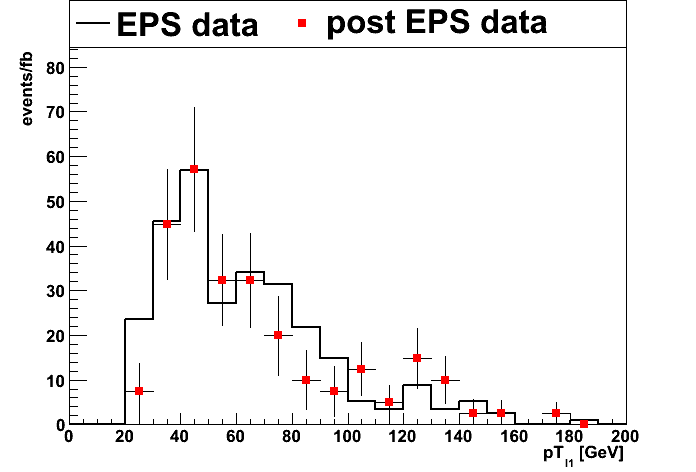
\includegraphics[width=.32\textwidth]{lp_figures/postEPSvalid/hm0/lep1pt_ww1j.png}}
\subfigure[]{
\centering
\label{subfig:lp_lep2pt_ww1j}
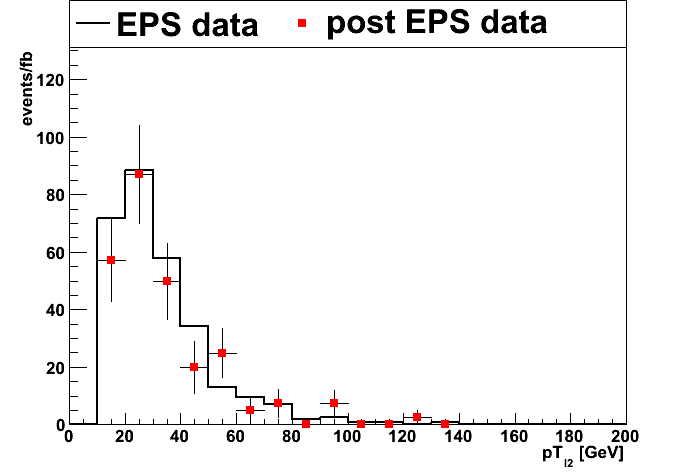
\includegraphics[width=.32\textwidth]{lp_figures/postEPSvalid/hm0/lep2pt_ww1j.png}}
\subfigure[]{
\centering
\label{subfig:lp_jet1pt_ww1j}
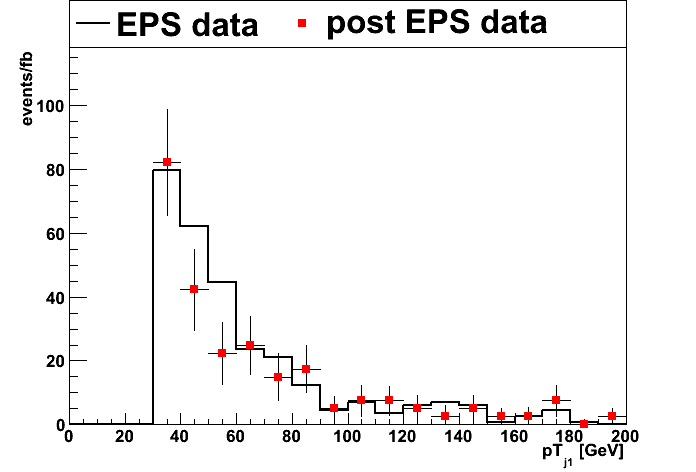
\includegraphics[width=.32\textwidth]{lp_figures/postEPSvalid/hm0/jet1pt_ww1j.png}}\\
\subfigure[]{
\centering
\label{subfig:lp_pmet_ww1j}
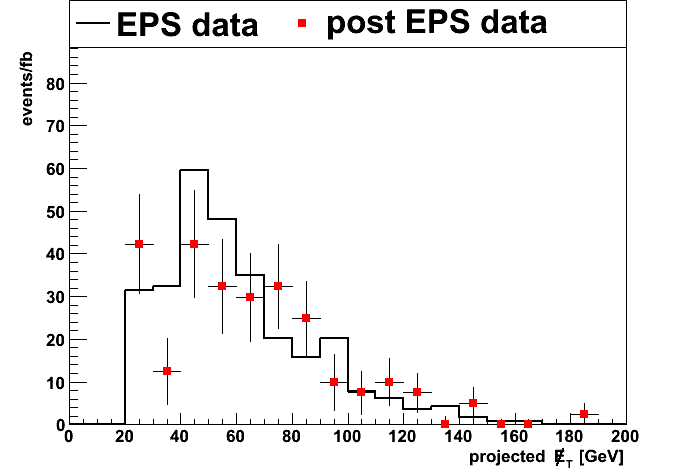
\includegraphics[width=.32\textwidth]{lp_figures/postEPSvalid/hm0/pmet_ww1j.png}}
\subfigure[]{
\centering
\label{subfig:lp_pTrackMet_ww1j}
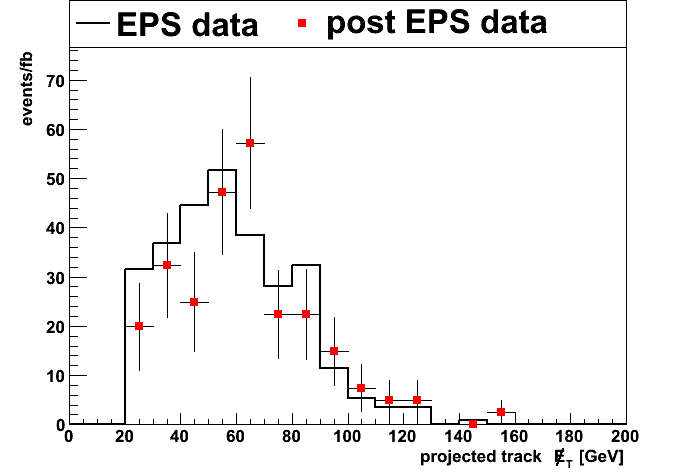
\includegraphics[width=.32\textwidth]{lp_figures/postEPSvalid/hm0/pTrackMet_ww1j.png}}
\subfigure[]{
\centering
\label{subfig:lp_mt_ww1j}
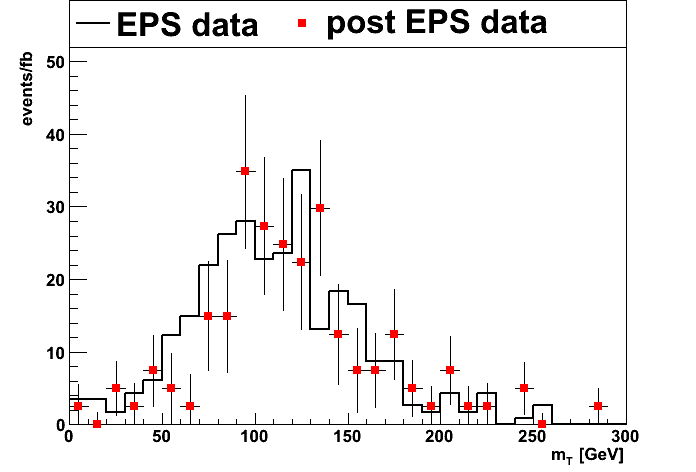
\includegraphics[width=.32\textwidth]{lp_figures/postEPSvalid/hm0/mt_ww1j.png}}
\caption{EPS and post-EPS data comparison: 1-jet bin, all final states. 
\subref{subfig:lp_lep1pt_ww1j} leading lepton $p_T$;
\subref{subfig:lp_lep2pt_ww1j} trailing lepton $p_T$;
\subref{subfig:lp_jet1pt_ww1j} leading jet $p_T$;
\subref{subfig:lp_pmet_ww1j} projected MET;
\subref{subfig:lp_pTrackMet_ww1j} projected track-MET;
\subref{subfig:lp_mt_ww1j} transverse mass of dilepton-MET system.
}
\label{fig:lp_ww1j_lepjetmet}
\end{figure}

\clearpage

\begin{figure}[!hbtp]
\centering
\subfigure[]{
\centering
\label{subfig:lp_dPhi_ww2j}
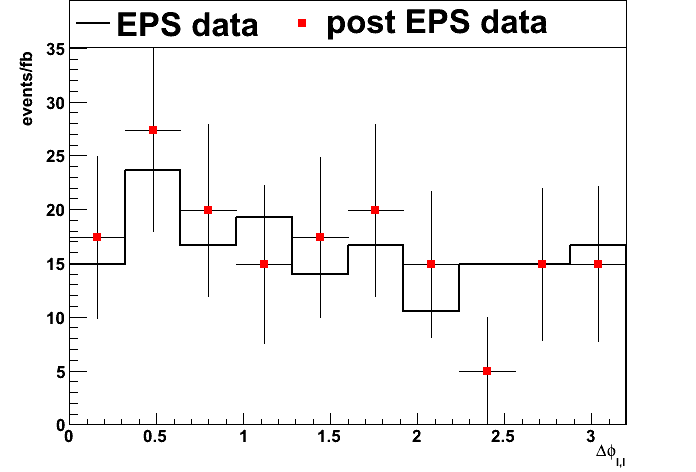
\includegraphics[width=.32\textwidth]{lp_figures/postEPSvalid/hm0/dPhi_ww2j.png}}
\subfigure[]{
\centering
\label{subfig:lp_dilepmass_ww2j}
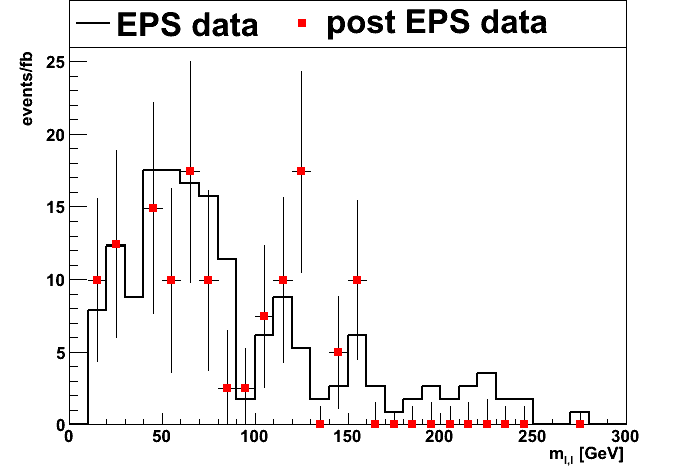
\includegraphics[width=.32\textwidth]{lp_figures/postEPSvalid/hm0/dilepmass_ww2j.png}}\\
\subfigure[]{
\centering
\label{subfig:lp_dileppt_ww2j}
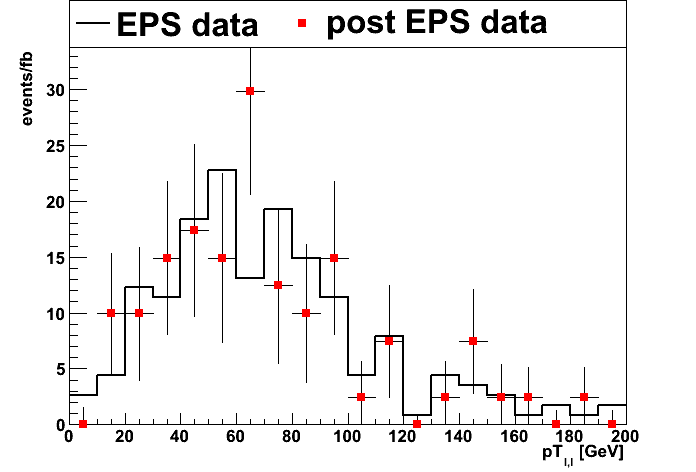
\includegraphics[width=.32\textwidth]{lp_figures/postEPSvalid/hm0/dileppt_ww2j.png}}
\subfigure[]{
\centering
\label{subfig:lp_type_ww2j}
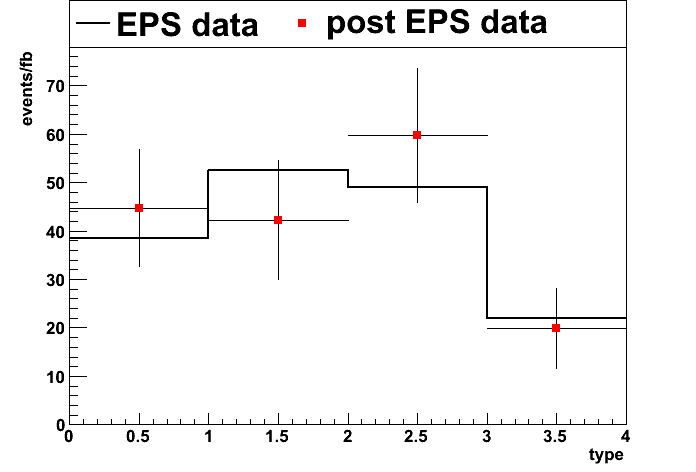
\includegraphics[width=.32\textwidth]{lp_figures/postEPSvalid/hm0/type_ww2j.png}}
\caption{EPS and post-EPS data comparison: 2-jet bin, all final states. 
\subref{subfig:lp_dPhi_ww2j} $\Delta\phi$ between the two leptons;
\subref{subfig:lp_dilepmass_ww2j} di-lepton invariant mass;
\subref{subfig:lp_dileppt_ww2j} di-lepton transverse momentum;
\subref{subfig:lp_type_ww2j} di-lepton type ($\mu\mu$=0, $\mu e$=2, $e\mu$=2, $ee$=3).
}
\label{fig:lp_ww2j_dilep}
\end{figure}

\begin{figure}[!hbtp]
\centering
\subfigure[]{
\centering
\label{subfig:lp_lep1pt_ww2j}
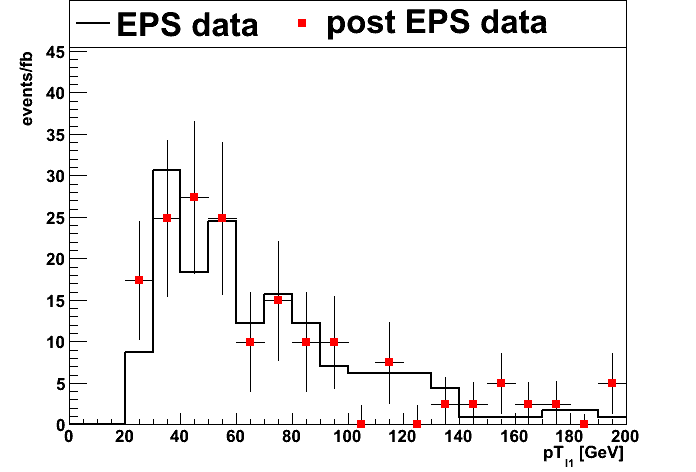
\includegraphics[width=.32\textwidth]{lp_figures/postEPSvalid/hm0/lep1pt_ww2j.png}}
\subfigure[]{
\centering
\label{subfig:lp_lep2pt_ww2j}
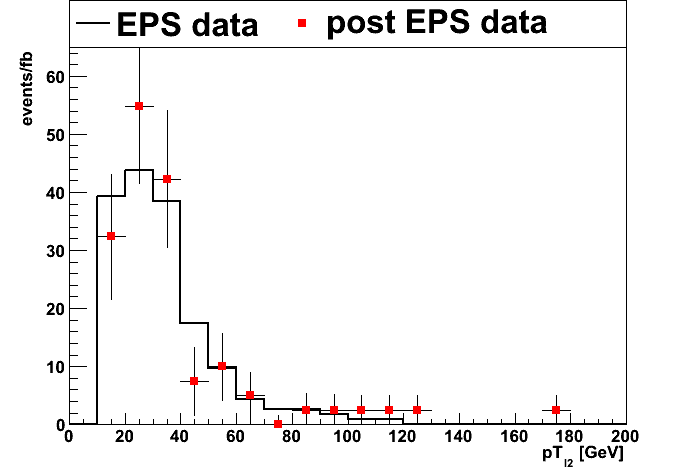
\includegraphics[width=.32\textwidth]{lp_figures/postEPSvalid/hm0/lep2pt_ww2j.png}}
\subfigure[]{
\centering
\label{subfig:lp_jet1pt_ww2j}
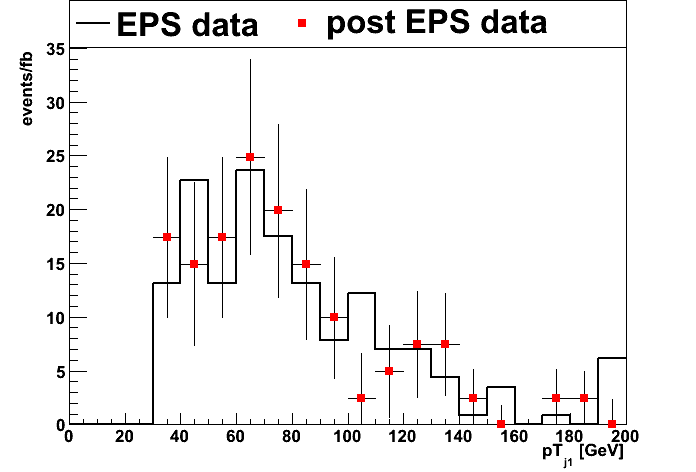
\includegraphics[width=.32\textwidth]{lp_figures/postEPSvalid/hm0/jet1pt_ww2j.png}}\\
\subfigure[]{
\centering
\label{subfig:lp_pmet_ww2j}
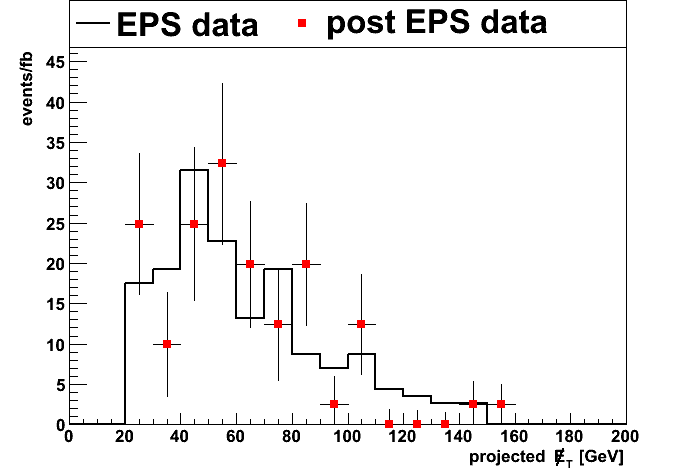
\includegraphics[width=.32\textwidth]{lp_figures/postEPSvalid/hm0/pmet_ww2j.png}}
\subfigure[]{
\centering
\label{subfig:lp_pTrackMet_ww2j}
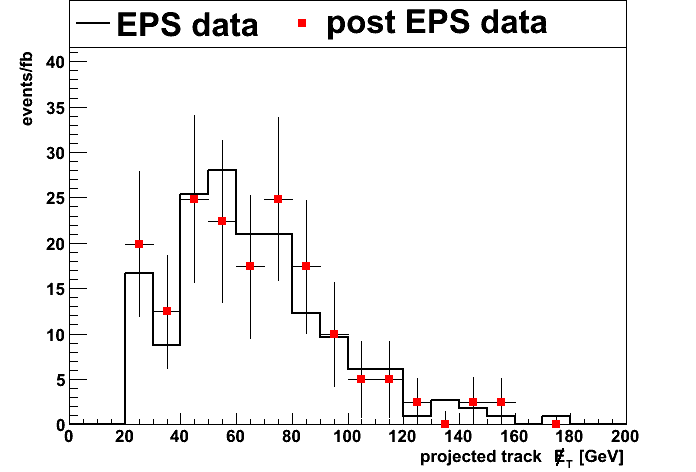
\includegraphics[width=.32\textwidth]{lp_figures/postEPSvalid/hm0/pTrackMet_ww2j.png}}
\subfigure[]{
\centering
\label{subfig:lp_mt_ww2j}
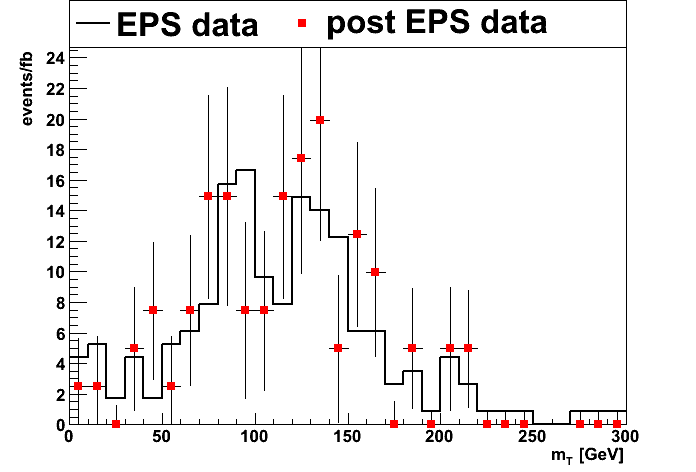
\includegraphics[width=.32\textwidth]{lp_figures/postEPSvalid/hm0/mt_ww2j.png}}
\caption{EPS and post-EPS data comparison: 2-jet bin, all final states. 
\subref{subfig:lp_lep1pt_ww2j} leading lepton $p_T$;
\subref{subfig:lp_lep2pt_ww2j} trailing lepton $p_T$;
\subref{subfig:lp_jet1pt_ww2j} leading jet $p_T$;
\subref{subfig:lp_pmet_ww2j} projected MET;
\subref{subfig:lp_pTrackMet_ww2j} projected track-MET;
\subref{subfig:lp_mt_ww2j} transverse mass of dilepton-MET system.
}
\label{fig:lp_ww2j_lepjetmet}
\end{figure}

\clearpage


    \subsection{MVA output plots}
    \label{app:lp_mvaplots}
    \subsubsection{EPS distributions}

This section contains the MVA output plots for the EPS dataset for $m_H$=115, 120, 130, 140, 150, 160, 200 GeV analyses split in opposte and same flavor, 
0-jet and 1-jet bin (Figures~\ref{fig:lp_mva_115_EPS}-\ref{fig:lp_mva_200_EPS}).

\begin{figure}[!hbtp]
\centering
\subfigure[]{
\centering
\label{subfig:lp_mva_115_0j_of_EPS}
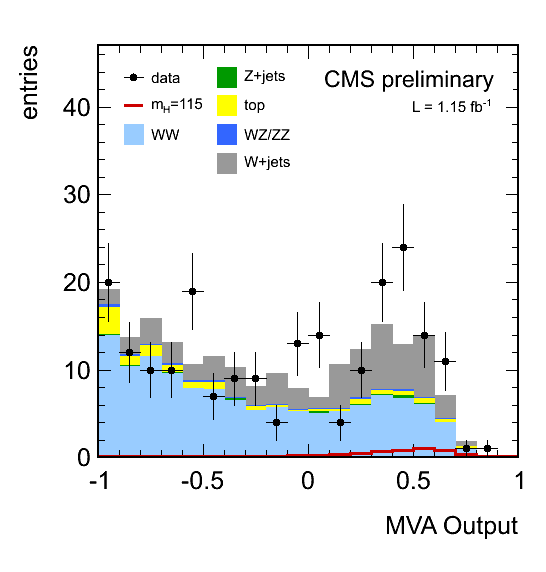
\includegraphics[width=.40\textwidth]{lp_figures/histo_mva_115_0j_of_EPS.png}}
\subfigure[]{
\centering
\label{subfig:lp_mva_115_0j_sf_EPS}
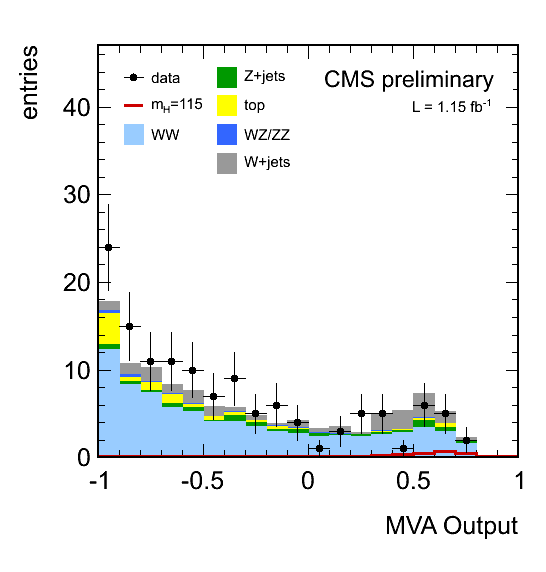
\includegraphics[width=.40\textwidth]{lp_figures/histo_mva_115_0j_sf_EPS.png}}\\
\subfigure[]{
\centering
\label{subfig:lp_mva_115_1j_of_EPS}
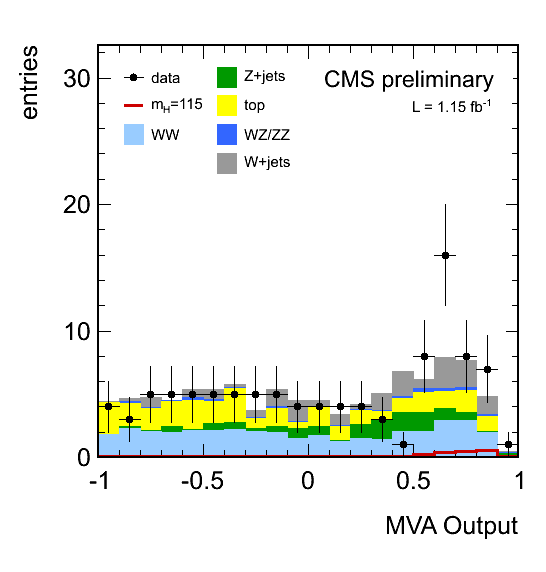
\includegraphics[width=.40\textwidth]{lp_figures/histo_mva_115_1j_of_EPS.png}}
\subfigure[]{
\centering
\label{subfig:lp_mva_115_1j_sf_EPS}
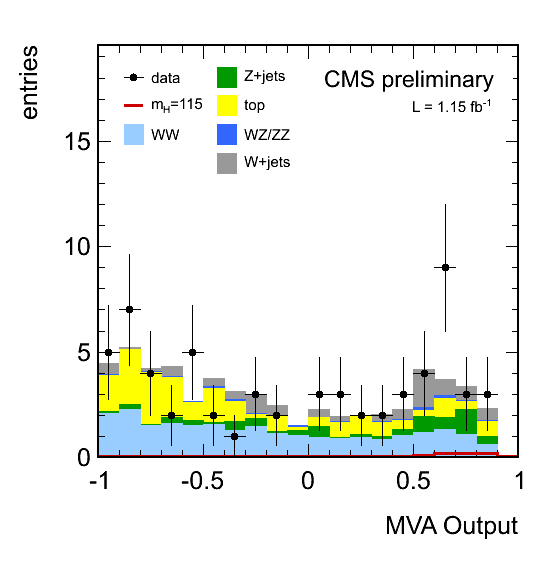
\includegraphics[width=.40\textwidth]{lp_figures/histo_mva_115_1j_sf_EPS.png}}
\caption{
MVA output for $m_H$=115 GeV EPS analysis: 
0-jet OF \subref{subfig:lp_mva_115_0j_of_EPS},
0-jet SF \subref{subfig:lp_mva_115_0j_sf_EPS},
1-jet OF \subref{subfig:lp_mva_115_1j_of_EPS},
1-jet SF \subref{subfig:lp_mva_115_1j_sf_EPS}
.}
\label{fig:lp_mva_115_EPS}
\end{figure}

\begin{figure}[!hbtp]
\centering
\subfigure[]{
\centering
\label{subfig:lp_mva_120_0j_of_EPS}
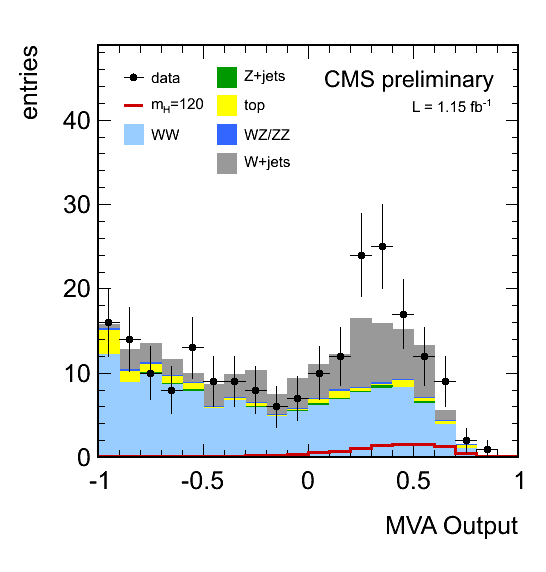
\includegraphics[width=.40\textwidth]{lp_figures/histo_mva_120_0j_of_EPS.png}}
\subfigure[]{
\centering
\label{subfig:lp_mva_120_0j_sf_EPS}
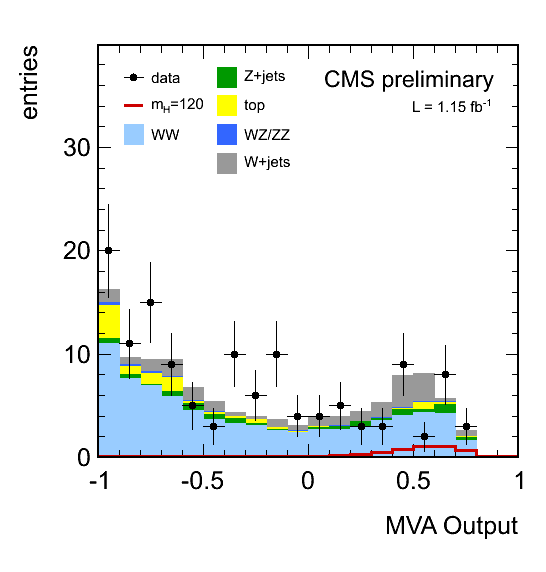
\includegraphics[width=.40\textwidth]{lp_figures/histo_mva_120_0j_sf_EPS.png}}\\
\subfigure[]{
\centering
\label{subfig:lp_mva_120_1j_of_EPS}
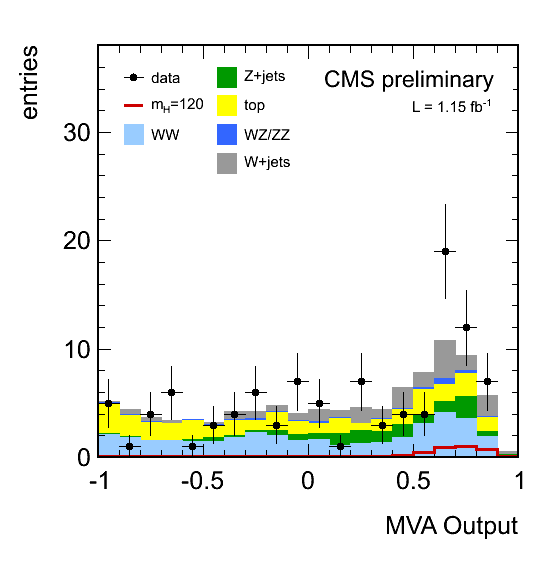
\includegraphics[width=.40\textwidth]{lp_figures/histo_mva_120_1j_of_EPS.png}}
\subfigure[]{
\centering
\label{subfig:lp_mva_120_1j_sf_EPS}
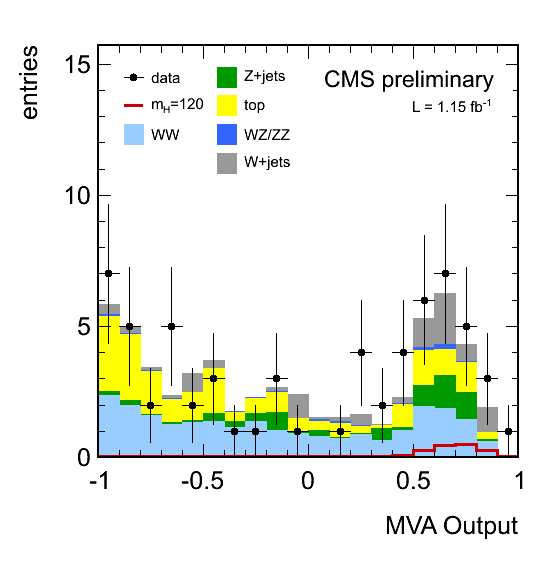
\includegraphics[width=.40\textwidth]{lp_figures/histo_mva_120_1j_sf_EPS.png}}
\caption{
MVA output for $m_H$=120 GeV EPS analysis: 
0-jet OF \subref{subfig:lp_mva_120_0j_of_EPS},
0-jet SF \subref{subfig:lp_mva_120_0j_sf_EPS},
1-jet OF \subref{subfig:lp_mva_120_1j_of_EPS},
1-jet SF \subref{subfig:lp_mva_120_1j_sf_EPS}
.}
\label{fig:lp_mva_120_EPS}
\end{figure}

\begin{figure}[!hbtp]
\centering
\subfigure[]{
\centering
\label{subfig:lp_mva_130_0j_of_EPS}
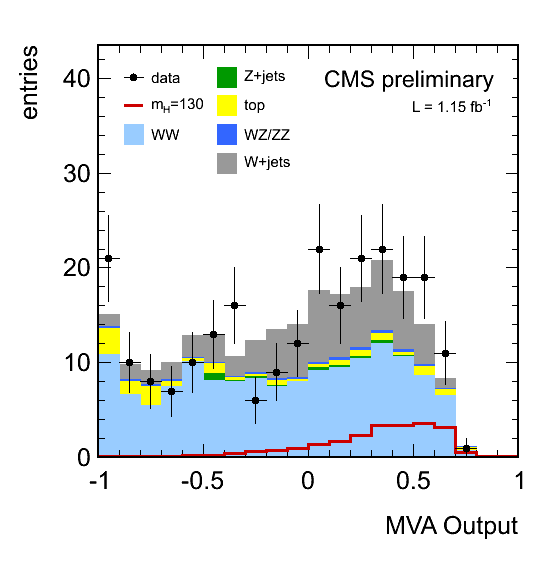
\includegraphics[width=.40\textwidth]{lp_figures/histo_mva_130_0j_of_EPS.png}}
\subfigure[]{
\centering
\label{subfig:lp_mva_130_0j_sf_EPS}
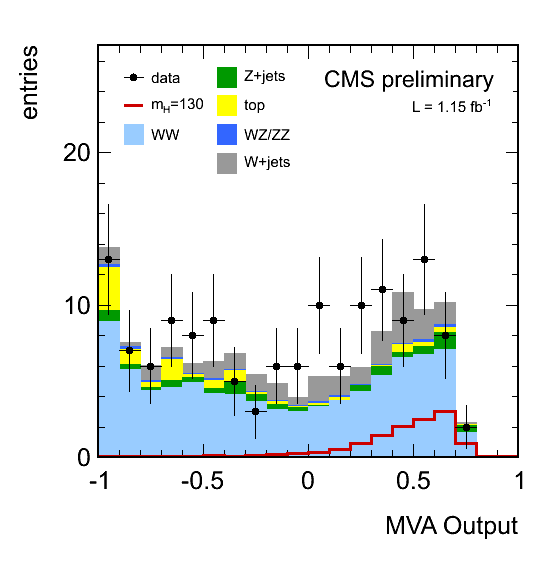
\includegraphics[width=.40\textwidth]{lp_figures/histo_mva_130_0j_sf_EPS.png}}\\
\subfigure[]{
\centering
\label{subfig:lp_mva_130_1j_of_EPS}
\includegraphics[width=.40\textwidth]{lp_figures/histo_mva_130_1j_of_EPS.png}}
\subfigure[]{
\centering
\label{subfig:lp_mva_130_1j_sf_EPS}
\includegraphics[width=.40\textwidth]{lp_figures/histo_mva_130_1j_sf_EPS.png}}
\caption{
MVA output for $m_H$=130 GeV EPS analysis: 
0-jet OF \subref{subfig:lp_mva_130_0j_of_EPS},
0-jet SF \subref{subfig:lp_mva_130_0j_sf_EPS},
1-jet OF \subref{subfig:lp_mva_130_1j_of_EPS},
1-jet SF \subref{subfig:lp_mva_130_1j_sf_EPS}
.}
\label{fig:lp_mva_130_EPS}
\end{figure}

\begin{figure}[!hbtp]
\centering
\subfigure[]{
\centering
\label{subfig:lp_mva_140_0j_of_EPS}
\includegraphics[width=.40\textwidth]{lp_figures/histo_mva_140_0j_of_EPS.png}}
\subfigure[]{
\centering
\label{subfig:lp_mva_140_0j_sf_EPS}
\includegraphics[width=.40\textwidth]{lp_figures/histo_mva_140_0j_sf_EPS.png}}\\
\subfigure[]{
\centering
\label{subfig:lp_mva_140_1j_of_EPS}
\includegraphics[width=.40\textwidth]{lp_figures/histo_mva_140_1j_of_EPS.png}}
\subfigure[]{
\centering
\label{subfig:lp_mva_140_1j_sf_EPS}
\includegraphics[width=.40\textwidth]{lp_figures/histo_mva_140_1j_sf_EPS.png}}
\caption{
MVA output for $m_H$=140 GeV EPS analysis: 
0-jet OF \subref{subfig:lp_mva_140_0j_of_EPS},
0-jet SF \subref{subfig:lp_mva_140_0j_sf_EPS},
1-jet OF \subref{subfig:lp_mva_140_1j_of_EPS},
1-jet SF \subref{subfig:lp_mva_140_1j_sf_EPS}
.}
\label{fig:lp_mva_140_EPS}
\end{figure}

\begin{figure}[!hbtp]
\centering
\subfigure[]{
\centering
\label{subfig:lp_mva_150_0j_of_EPS}
\includegraphics[width=.40\textwidth]{lp_figures/histo_mva_150_0j_of_EPS.png}}
\subfigure[]{
\centering
\label{subfig:lp_mva_150_0j_sf_EPS}
\includegraphics[width=.40\textwidth]{lp_figures/histo_mva_150_0j_sf_EPS.png}}\\
\subfigure[]{
\centering
\label{subfig:lp_mva_150_1j_of_EPS}
\includegraphics[width=.40\textwidth]{lp_figures/histo_mva_150_1j_of_EPS.png}}
\subfigure[]{
\centering
\label{subfig:lp_mva_150_1j_sf_EPS}
\includegraphics[width=.40\textwidth]{lp_figures/histo_mva_150_1j_sf_EPS.png}}
\caption{
MVA output for $m_H$=150 GeV EPS analysis: 
0-jet OF \subref{subfig:lp_mva_150_0j_of_EPS},
0-jet SF \subref{subfig:lp_mva_150_0j_sf_EPS},
1-jet OF \subref{subfig:lp_mva_150_1j_of_EPS},
1-jet SF \subref{subfig:lp_mva_150_1j_sf_EPS}
.}
\label{fig:lp_mva_150_EPS}
\end{figure}

\begin{figure}[!hbtp]
\centering
\subfigure[]{
\centering
\label{subfig:lp_mva_160_0j_of_EPS}
\includegraphics[width=.40\textwidth]{lp_figures/histo_mva_160_0j_of_EPS.png}}
\subfigure[]{
\centering
\label{subfig:lp_mva_160_0j_sf_EPS}
\includegraphics[width=.40\textwidth]{lp_figures/histo_mva_160_0j_sf_EPS.png}}\\
\subfigure[]{
\centering
\label{subfig:lp_mva_160_1j_of_EPS}
\includegraphics[width=.40\textwidth]{lp_figures/histo_mva_160_1j_of_EPS.png}}
\subfigure[]{
\centering
\label{subfig:lp_mva_160_1j_sf_EPS}
\includegraphics[width=.40\textwidth]{lp_figures/histo_mva_160_1j_sf_EPS.png}}
\caption{
MVA output for $m_H$=160 GeV EPS analysis: 
0-jet OF \subref{subfig:lp_mva_160_0j_of_EPS},
0-jet SF \subref{subfig:lp_mva_160_0j_sf_EPS},
1-jet OF \subref{subfig:lp_mva_160_1j_of_EPS},
1-jet SF \subref{subfig:lp_mva_160_1j_sf_EPS}
.}
\label{fig:lp_mva_160_EPS}
\end{figure}

\begin{figure}[!hbtp]
\centering
\subfigure[]{
\centering
\label{subfig:lp_mva_200_0j_of_EPS}
\includegraphics[width=.40\textwidth]{lp_figures/histo_mva_200_0j_of_EPS.png}}
\subfigure[]{
\centering
\label{subfig:lp_mva_200_0j_sf_EPS}
\includegraphics[width=.40\textwidth]{lp_figures/histo_mva_200_0j_sf_EPS.png}}\\
\subfigure[]{
\centering
\label{subfig:lp_mva_200_1j_of_EPS}
\includegraphics[width=.40\textwidth]{lp_figures/histo_mva_200_1j_of_EPS.png}}
\subfigure[]{
\centering
\label{subfig:lp_mva_200_1j_sf_EPS}
\includegraphics[width=.40\textwidth]{lp_figures/histo_mva_200_1j_sf_EPS.png}}
\caption{
MVA output for $m_H$=200 GeV EPS analysis: 
0-jet OF \subref{subfig:lp_mva_200_0j_of_EPS},
0-jet SF \subref{subfig:lp_mva_200_0j_sf_EPS},
1-jet OF \subref{subfig:lp_mva_200_1j_of_EPS},
1-jet SF \subref{subfig:lp_mva_200_1j_sf_EPS}
.}
\label{fig:lp_mva_200_EPS}
\end{figure}

\clearpage

    \subsection{Post-EPS distributions}

This section contains the MVA output plots for the post-EPS dataset for $m_H$=115, 120, 130, 140, 150, 160, 200 GeV analyses split in opposte and same flavor, 
0-jet and 1-jet bin (Figures~\ref{fig:lp_mva_115_POSTEPS}-\ref{fig:lp_mva_200_POSTEPS}).

\begin{figure}[!hbtp]
\centering
\subfigure[]{
\centering
\label{subfig:lp_mva_115_0j_of_POSTEPS}
\includegraphics[width=.40\textwidth]{lp_figures/histo_mva_115_0j_of_POSTEPS.png}}
\subfigure[]{
\centering
\label{subfig:lp_mva_115_0j_sf_POSTEPS}
\includegraphics[width=.40\textwidth]{lp_figures/histo_mva_115_0j_sf_POSTEPS.png}}\\
\subfigure[]{
\centering
\label{subfig:lp_mva_115_1j_of_POSTEPS}
\includegraphics[width=.40\textwidth]{lp_figures/histo_mva_115_1j_of_POSTEPS.png}}
\subfigure[]{
\centering
\label{subfig:lp_mva_115_1j_sf_POSTEPS}
\includegraphics[width=.40\textwidth]{lp_figures/histo_mva_115_1j_sf_POSTEPS.png}}
\caption{
MVA output for $m_H$=115 GeV post-EPS analysis: 
0-jet OF \subref{subfig:lp_mva_115_0j_of_POSTEPS},
0-jet SF \subref{subfig:lp_mva_115_0j_sf_POSTEPS},
1-jet OF \subref{subfig:lp_mva_115_1j_of_POSTEPS},
1-jet SF \subref{subfig:lp_mva_115_1j_sf_POSTEPS}
.}
\label{fig:lp_mva_115_POSTEPS}
\end{figure}

\begin{figure}[!hbtp]
\centering
\subfigure[]{
\centering
\label{subfig:lp_mva_120_0j_of_POSTEPS}
\includegraphics[width=.40\textwidth]{lp_figures/histo_mva_120_0j_of_POSTEPS.png}}
\subfigure[]{
\centering
\label{subfig:lp_mva_120_0j_sf_POSTEPS}
\includegraphics[width=.40\textwidth]{lp_figures/histo_mva_120_0j_sf_POSTEPS.png}}\\
\subfigure[]{
\centering
\label{subfig:lp_mva_120_1j_of_POSTEPS}
\includegraphics[width=.40\textwidth]{lp_figures/histo_mva_120_1j_of_POSTEPS.png}}
\subfigure[]{
\centering
\label{subfig:lp_mva_120_1j_sf_POSTEPS}
\includegraphics[width=.40\textwidth]{lp_figures/histo_mva_120_1j_sf_POSTEPS.png}}
\caption{
MVA output for $m_H$=120 GeV post-EPS analysis: 
0-jet OF \subref{subfig:lp_mva_120_0j_of_POSTEPS},
0-jet SF \subref{subfig:lp_mva_120_0j_sf_POSTEPS},
1-jet OF \subref{subfig:lp_mva_120_1j_of_POSTEPS},
1-jet SF \subref{subfig:lp_mva_120_1j_sf_POSTEPS}
.}
\label{fig:lp_mva_120_POSTEPS}
\end{figure}

\begin{figure}[!hbtp]
\centering
\subfigure[]{
\centering
\label{subfig:lp_mva_130_0j_of_POSTEPS}
\includegraphics[width=.40\textwidth]{lp_figures/histo_mva_130_0j_of_POSTEPS.png}}
\subfigure[]{
\centering
\label{subfig:lp_mva_130_0j_sf_POSTEPS}
\includegraphics[width=.40\textwidth]{lp_figures/histo_mva_130_0j_sf_POSTEPS.png}}\\
\subfigure[]{
\centering
\label{subfig:lp_mva_130_1j_of_POSTEPS}
\includegraphics[width=.40\textwidth]{lp_figures/histo_mva_130_1j_of_POSTEPS.png}}
\subfigure[]{
\centering
\label{subfig:lp_mva_130_1j_sf_POSTEPS}
\includegraphics[width=.40\textwidth]{lp_figures/histo_mva_130_1j_sf_POSTEPS.png}}
\caption{
MVA output for $m_H$=130 GeV post-EPS analysis: 
0-jet OF \subref{subfig:lp_mva_130_0j_of_POSTEPS},
0-jet SF \subref{subfig:lp_mva_130_0j_sf_POSTEPS},
1-jet OF \subref{subfig:lp_mva_130_1j_of_POSTEPS},
1-jet SF \subref{subfig:lp_mva_130_1j_sf_POSTEPS}
.}
\label{fig:lp_mva_130_POSTEPS}
\end{figure}

\begin{figure}[!hbtp]
\centering
\subfigure[]{
\centering
\label{subfig:lp_mva_140_0j_of_POSTEPS}
\includegraphics[width=.40\textwidth]{lp_figures/histo_mva_140_0j_of_POSTEPS.png}}
\subfigure[]{
\centering
\label{subfig:lp_mva_140_0j_sf_POSTEPS}
\includegraphics[width=.40\textwidth]{lp_figures/histo_mva_140_0j_sf_POSTEPS.png}}\\
\subfigure[]{
\centering
\label{subfig:lp_mva_140_1j_of_POSTEPS}
\includegraphics[width=.40\textwidth]{lp_figures/histo_mva_140_1j_of_POSTEPS.png}}
\subfigure[]{
\centering
\label{subfig:lp_mva_140_1j_sf_POSTEPS}
\includegraphics[width=.40\textwidth]{lp_figures/histo_mva_140_1j_sf_POSTEPS.png}}
\caption{
MVA output for $m_H$=140 GeV post-EPS analysis: 
0-jet OF \subref{subfig:lp_mva_140_0j_of_POSTEPS},
0-jet SF \subref{subfig:lp_mva_140_0j_sf_POSTEPS},
1-jet OF \subref{subfig:lp_mva_140_1j_of_POSTEPS},
1-jet SF \subref{subfig:lp_mva_140_1j_sf_POSTEPS}
.}
\label{fig:lp_mva_140_POSTEPS}
\end{figure}

\begin{figure}[!hbtp]
\centering
\subfigure[]{
\centering
\label{subfig:lp_mva_150_0j_of_POSTEPS}
\includegraphics[width=.40\textwidth]{lp_figures/histo_mva_150_0j_of_POSTEPS.png}}
\subfigure[]{
\centering
\label{subfig:lp_mva_150_0j_sf_POSTEPS}
\includegraphics[width=.40\textwidth]{lp_figures/histo_mva_150_0j_sf_POSTEPS.png}}\\
\subfigure[]{
\centering
\label{subfig:lp_mva_150_1j_of_POSTEPS}
\includegraphics[width=.40\textwidth]{lp_figures/histo_mva_150_1j_of_POSTEPS.png}}
\subfigure[]{
\centering
\label{subfig:lp_mva_150_1j_sf_POSTEPS}
\includegraphics[width=.40\textwidth]{lp_figures/histo_mva_150_1j_sf_POSTEPS.png}}
\caption{
MVA output for $m_H$=150 GeV post-EPS analysis: 
0-jet OF \subref{subfig:lp_mva_150_0j_of_POSTEPS},
0-jet SF \subref{subfig:lp_mva_150_0j_sf_POSTEPS},
1-jet OF \subref{subfig:lp_mva_150_1j_of_POSTEPS},
1-jet SF \subref{subfig:lp_mva_150_1j_sf_POSTEPS}
.}
\label{fig:lp_mva_150_POSTEPS}
\end{figure}

\begin{figure}[!hbtp]
\centering
\subfigure[]{
\centering
\label{subfig:lp_mva_160_0j_of_POSTEPS}
\includegraphics[width=.40\textwidth]{lp_figures/histo_mva_160_0j_of_POSTEPS.png}}
\subfigure[]{
\centering
\label{subfig:lp_mva_160_0j_sf_POSTEPS}
\includegraphics[width=.40\textwidth]{lp_figures/histo_mva_160_0j_sf_POSTEPS.png}}\\
\subfigure[]{
\centering
\label{subfig:lp_mva_160_1j_of_POSTEPS}
\includegraphics[width=.40\textwidth]{lp_figures/histo_mva_160_1j_of_POSTEPS.png}}
\subfigure[]{
\centering
\label{subfig:lp_mva_160_1j_sf_POSTEPS}
\includegraphics[width=.40\textwidth]{lp_figures/histo_mva_160_1j_sf_POSTEPS.png}}
\caption{
MVA output for $m_H$=160 GeV post-EPS analysis: 
0-jet OF \subref{subfig:lp_mva_160_0j_of_POSTEPS},
0-jet SF \subref{subfig:lp_mva_160_0j_sf_POSTEPS},
1-jet OF \subref{subfig:lp_mva_160_1j_of_POSTEPS},
1-jet SF \subref{subfig:lp_mva_160_1j_sf_POSTEPS}
.}
\label{fig:lp_mva_160_POSTEPS}
\end{figure}

\begin{figure}[!hbtp]
\centering
\subfigure[]{
\centering
\label{subfig:lp_mva_200_0j_of_POSTEPS}
\includegraphics[width=.40\textwidth]{lp_figures/histo_mva_200_0j_of_POSTEPS.png}}
\subfigure[]{
\centering
\label{subfig:lp_mva_200_0j_sf_POSTEPS}
\includegraphics[width=.40\textwidth]{lp_figures/histo_mva_200_0j_sf_POSTEPS.png}}\\
\subfigure[]{
\centering
\label{subfig:lp_mva_200_1j_of_POSTEPS}
\includegraphics[width=.40\textwidth]{lp_figures/histo_mva_200_1j_of_POSTEPS.png}}
\subfigure[]{
\centering
\label{subfig:lp_mva_200_1j_sf_POSTEPS}
\includegraphics[width=.40\textwidth]{lp_figures/histo_mva_200_1j_sf_POSTEPS.png}}
\caption{
MVA output for $m_H$=200 GeV post-EPS analysis: 
0-jet OF \subref{subfig:lp_mva_200_0j_of_POSTEPS},
0-jet SF \subref{subfig:lp_mva_200_0j_sf_POSTEPS},
1-jet OF \subref{subfig:lp_mva_200_1j_of_POSTEPS},
1-jet SF \subref{subfig:lp_mva_200_1j_sf_POSTEPS}
.}
\label{fig:lp_mva_200_POSTEPS}
\end{figure}

\clearpage

    \subsection{LP distributions}

This section contains the MVA output plots for the LP dataset for $m_H$=115, 120, 130, 140, 150, 160, 200 GeV analyses split in opposte and same flavor, 
0-jet and 1-jet bin (Figures~\ref{fig:lp_mva_115}-\ref{fig:lp_mva_200}).

\begin{figure}[!hbtp]
\centering
\subfigure[]{
\centering
\label{subfig:lp_mva_115_0j_of}
\includegraphics[width=.40\textwidth]{lp_figures/histo_mva_115_0j_of.png}}
\subfigure[]{
\centering
\label{subfig:lp_mva_115_0j_sf}
\includegraphics[width=.40\textwidth]{lp_figures/histo_mva_115_0j_sf.png}}\\
\subfigure[]{
\centering
\label{subfig:lp_mva_115_1j_of}
\includegraphics[width=.40\textwidth]{lp_figures/histo_mva_115_1j_of.png}}
\subfigure[]{
\centering
\label{subfig:lp_mva_115_1j_sf}
\includegraphics[width=.40\textwidth]{lp_figures/histo_mva_115_1j_sf.png}}
\caption{
MVA output for $m_H$=115 GeV LP analysis: 
0-jet OF \subref{subfig:lp_mva_115_0j_of},
0-jet SF \subref{subfig:lp_mva_115_0j_sf},
1-jet OF \subref{subfig:lp_mva_115_1j_of},
1-jet SF \subref{subfig:lp_mva_115_1j_sf}
.}
\label{fig:lp_mva_115}
\end{figure}

\begin{figure}[!hbtp]
\centering
\subfigure[]{
\centering
\label{subfig:lp_mva_120_0j_of}
\includegraphics[width=.40\textwidth]{lp_figures/histo_mva_120_0j_of.png}}
\subfigure[]{
\centering
\label{subfig:lp_mva_120_0j_sf}
\includegraphics[width=.40\textwidth]{lp_figures/histo_mva_120_0j_sf.png}}\\
\subfigure[]{
\centering
\label{subfig:lp_mva_120_1j_of}
\includegraphics[width=.40\textwidth]{lp_figures/histo_mva_120_1j_of.png}}
\subfigure[]{
\centering
\label{subfig:lp_mva_120_1j_sf}
\includegraphics[width=.40\textwidth]{lp_figures/histo_mva_120_1j_sf.png}}
\caption{
MVA output for $m_H$=120 GeV LP analysis: 
0-jet OF \subref{subfig:lp_mva_120_0j_of},
0-jet SF \subref{subfig:lp_mva_120_0j_sf},
1-jet OF \subref{subfig:lp_mva_120_1j_of},
1-jet SF \subref{subfig:lp_mva_120_1j_sf}
.}
\label{fig:lp_mva_120}
\end{figure}

\begin{figure}[!hbtp]
\centering
\subfigure[]{
\centering
\label{subfig:lp_mva_130_0j_of}
\includegraphics[width=.40\textwidth]{lp_figures/histo_mva_130_0j_of.png}}
\subfigure[]{
\centering
\label{subfig:lp_mva_130_0j_sf}
\includegraphics[width=.40\textwidth]{lp_figures/histo_mva_130_0j_sf.png}}\\
\subfigure[]{
\centering
\label{subfig:lp_mva_130_1j_of}
\includegraphics[width=.40\textwidth]{lp_figures/histo_mva_130_1j_of.png}}
\subfigure[]{
\centering
\label{subfig:lp_mva_130_1j_sf}
\includegraphics[width=.40\textwidth]{lp_figures/histo_mva_130_1j_sf.png}}
\caption{
MVA output for $m_H$=130 GeV LP analysis: 
0-jet OF \subref{subfig:lp_mva_130_0j_of},
0-jet SF \subref{subfig:lp_mva_130_0j_sf},
1-jet OF \subref{subfig:lp_mva_130_1j_of},
1-jet SF \subref{subfig:lp_mva_130_1j_sf}
.}
\label{fig:lp_mva_130}
\end{figure}

\begin{figure}[!hbtp]
\centering
\subfigure[]{
\centering
\label{subfig:lp_mva_140_0j_of}
\includegraphics[width=.40\textwidth]{lp_figures/histo_mva_140_0j_of.png}}
\subfigure[]{
\centering
\label{subfig:lp_mva_140_0j_sf}
\includegraphics[width=.40\textwidth]{lp_figures/histo_mva_140_0j_sf.png}}\\
\subfigure[]{
\centering
\label{subfig:lp_mva_140_1j_of}
\includegraphics[width=.40\textwidth]{lp_figures/histo_mva_140_1j_of.png}}
\subfigure[]{
\centering
\label{subfig:lp_mva_140_1j_sf}
\includegraphics[width=.40\textwidth]{lp_figures/histo_mva_140_1j_sf.png}}
\caption{
MVA output for $m_H$=140 GeV LP analysis: 
0-jet OF \subref{subfig:lp_mva_140_0j_of},
0-jet SF \subref{subfig:lp_mva_140_0j_sf},
1-jet OF \subref{subfig:lp_mva_140_1j_of},
1-jet SF \subref{subfig:lp_mva_140_1j_sf}
.}
\label{fig:lp_mva_140}
\end{figure}

\begin{figure}[!hbtp]
\centering
\subfigure[]{
\centering
\label{subfig:lp_mva_150_0j_of}
\includegraphics[width=.40\textwidth]{lp_figures/histo_mva_150_0j_of.png}}
\subfigure[]{
\centering
\label{subfig:lp_mva_150_0j_sf}
\includegraphics[width=.40\textwidth]{lp_figures/histo_mva_150_0j_sf.png}}\\
\subfigure[]{
\centering
\label{subfig:lp_mva_150_1j_of}
\includegraphics[width=.40\textwidth]{lp_figures/histo_mva_150_1j_of.png}}
\subfigure[]{
\centering
\label{subfig:lp_mva_150_1j_sf}
\includegraphics[width=.40\textwidth]{lp_figures/histo_mva_150_1j_sf.png}}
\caption{
MVA output for $m_H$=150 GeV LP analysis: 
0-jet OF \subref{subfig:lp_mva_150_0j_of},
0-jet SF \subref{subfig:lp_mva_150_0j_sf},
1-jet OF \subref{subfig:lp_mva_150_1j_of},
1-jet SF \subref{subfig:lp_mva_150_1j_sf}
.}
\label{fig:lp_mva_150}
\end{figure}

\begin{figure}[!hbtp]
\centering
\subfigure[]{
\centering
\label{subfig:lp_mva_160_0j_of}
\includegraphics[width=.40\textwidth]{lp_figures/histo_mva_160_0j_of.png}}
\subfigure[]{
\centering
\label{subfig:lp_mva_160_0j_sf}
\includegraphics[width=.40\textwidth]{lp_figures/histo_mva_160_0j_sf.png}}\\
\subfigure[]{
\centering
\label{subfig:lp_mva_160_1j_of}
\includegraphics[width=.40\textwidth]{lp_figures/histo_mva_160_1j_of.png}}
\subfigure[]{
\centering
\label{subfig:lp_mva_160_1j_sf}
\includegraphics[width=.40\textwidth]{lp_figures/histo_mva_160_1j_sf.png}}
\caption{
MVA output for $m_H$=160 GeV LP analysis: 
0-jet OF \subref{subfig:lp_mva_160_0j_of},
0-jet SF \subref{subfig:lp_mva_160_0j_sf},
1-jet OF \subref{subfig:lp_mva_160_1j_of},
1-jet SF \subref{subfig:lp_mva_160_1j_sf}
.}
\label{fig:lp_mva_160}
\end{figure}

\begin{figure}[!hbtp]
\centering
\subfigure[]{
\centering
\label{subfig:lp_mva_200_0j_of}
\includegraphics[width=.40\textwidth]{lp_figures/histo_mva_200_0j_of.png}}
\subfigure[]{
\centering
\label{subfig:lp_mva_200_0j_sf}
\includegraphics[width=.40\textwidth]{lp_figures/histo_mva_200_0j_sf.png}}\\
\subfigure[]{
\centering
\label{subfig:lp_mva_200_1j_of}
\includegraphics[width=.40\textwidth]{lp_figures/histo_mva_200_1j_of.png}}
\subfigure[]{
\centering
\label{subfig:lp_mva_200_1j_sf}
\includegraphics[width=.40\textwidth]{lp_figures/histo_mva_200_1j_sf.png}}
\caption{
MVA output for $m_H$=200 GeV LP analysis: 
0-jet OF \subref{subfig:lp_mva_200_0j_of},
0-jet SF \subref{subfig:lp_mva_200_0j_sf},
1-jet OF \subref{subfig:lp_mva_200_1j_of},
1-jet SF \subref{subfig:lp_mva_200_1j_sf}
.}
\label{fig:lp_mva_200}
\end{figure}

\clearpage

    \subsubsection{LP distributions with $80<m_T<m_H$}

This section contains the MVA output plots for the LP dataset for $m_H$=115, 120, 130, 140, 150, 160, 200 GeV analyses split in opposte and same flavor, 
0-jet and 1-jet bin requiring a transverse mass value greater than 80 GeV and smaller than the considered Higgs mass 
(Figures~\ref{fig:lp_mva_115_MTCUTGT80}-\ref{fig:lp_mva_200_MTCUTGT80}).

\begin{figure}[!hbtp]
\centering
\subfigure[]{
\centering
\label{subfig:lp_mva_115_0j_of_MTCUTGT80}
\includegraphics[width=.40\textwidth]{lp_figures/histo_mva_115_0j_of_MTCUTGT80.png}}
\subfigure[]{
\centering
\label{subfig:lp_mva_115_0j_sf_MTCUTGT80}
\includegraphics[width=.40\textwidth]{lp_figures/histo_mva_115_0j_sf_MTCUTGT80.png}}\\
\subfigure[]{
\centering
\label{subfig:lp_mva_115_1j_of_MTCUTGT80}
\includegraphics[width=.40\textwidth]{lp_figures/histo_mva_115_1j_of_MTCUTGT80.png}}
\subfigure[]{
\centering
\label{subfig:lp_mva_115_1j_sf_MTCUTGT80}
\includegraphics[width=.40\textwidth]{lp_figures/histo_mva_115_1j_sf_MTCUTGT80.png}}
\caption{
MVA output for $m_H$=115 GeV LP ($80<m_T<m_H$) analysis: 
0-jet OF \subref{subfig:lp_mva_115_0j_of_MTCUTGT80},
0-jet SF \subref{subfig:lp_mva_115_0j_sf_MTCUTGT80},
1-jet OF \subref{subfig:lp_mva_115_1j_of_MTCUTGT80},
1-jet SF \subref{subfig:lp_mva_115_1j_sf_MTCUTGT80}
.}
\label{fig:lp_mva_115_MTCUTGT80}
\end{figure}

\begin{figure}[!hbtp]
\centering
\subfigure[]{
\centering
\label{subfig:lp_mva_120_0j_of_MTCUTGT80}
\includegraphics[width=.40\textwidth]{lp_figures/histo_mva_120_0j_of_MTCUTGT80.png}}
\subfigure[]{
\centering
\label{subfig:lp_mva_120_0j_sf_MTCUTGT80}
\includegraphics[width=.40\textwidth]{lp_figures/histo_mva_120_0j_sf_MTCUTGT80.png}}\\
\subfigure[]{
\centering
\label{subfig:lp_mva_120_1j_of_MTCUTGT80}
\includegraphics[width=.40\textwidth]{lp_figures/histo_mva_120_1j_of_MTCUTGT80.png}}
\subfigure[]{
\centering
\label{subfig:lp_mva_120_1j_sf_MTCUTGT80}
\includegraphics[width=.40\textwidth]{lp_figures/histo_mva_120_1j_sf_MTCUTGT80.png}}
\caption{
MVA output for $m_H$=120 GeV LP ($80<m_T<m_H$) analysis: 
0-jet OF \subref{subfig:lp_mva_120_0j_of_MTCUTGT80},
0-jet SF \subref{subfig:lp_mva_120_0j_sf_MTCUTGT80},
1-jet OF \subref{subfig:lp_mva_120_1j_of_MTCUTGT80},
1-jet SF \subref{subfig:lp_mva_120_1j_sf_MTCUTGT80}
.}
\label{fig:lp_mva_120_MTCUTGT80}
\end{figure}

\begin{figure}[!hbtp]
\centering
\subfigure[]{
\centering
\label{subfig:lp_mva_130_0j_of_MTCUTGT80}
\includegraphics[width=.40\textwidth]{lp_figures/histo_mva_130_0j_of_MTCUTGT80.png}}
\subfigure[]{
\centering
\label{subfig:lp_mva_130_0j_sf_MTCUTGT80}
\includegraphics[width=.40\textwidth]{lp_figures/histo_mva_130_0j_sf_MTCUTGT80.png}}\\
\subfigure[]{
\centering
\label{subfig:lp_mva_130_1j_of_MTCUTGT80}
\includegraphics[width=.40\textwidth]{lp_figures/histo_mva_130_1j_of_MTCUTGT80.png}}
\subfigure[]{
\centering
\label{subfig:lp_mva_130_1j_sf_MTCUTGT80}
\includegraphics[width=.40\textwidth]{lp_figures/histo_mva_130_1j_sf_MTCUTGT80.png}}
\caption{
MVA output for $m_H$=130 GeV LP ($80<m_T<m_H$) analysis: 
0-jet OF \subref{subfig:lp_mva_130_0j_of_MTCUTGT80},
0-jet SF \subref{subfig:lp_mva_130_0j_sf_MTCUTGT80},
1-jet OF \subref{subfig:lp_mva_130_1j_of_MTCUTGT80},
1-jet SF \subref{subfig:lp_mva_130_1j_sf_MTCUTGT80}
.}
\label{fig:lp_mva_130_MTCUTGT80}
\end{figure}

\begin{figure}[!hbtp]
\centering
\subfigure[]{
\centering
\label{subfig:lp_mva_140_0j_of_MTCUTGT80}
\includegraphics[width=.40\textwidth]{lp_figures/histo_mva_140_0j_of_MTCUTGT80.png}}
\subfigure[]{
\centering
\label{subfig:lp_mva_140_0j_sf_MTCUTGT80}
\includegraphics[width=.40\textwidth]{lp_figures/histo_mva_140_0j_sf_MTCUTGT80.png}}\\
\subfigure[]{
\centering
\label{subfig:lp_mva_140_1j_of_MTCUTGT80}
\includegraphics[width=.40\textwidth]{lp_figures/histo_mva_140_1j_of_MTCUTGT80.png}}
\subfigure[]{
\centering
\label{subfig:lp_mva_140_1j_sf_MTCUTGT80}
\includegraphics[width=.40\textwidth]{lp_figures/histo_mva_140_1j_sf_MTCUTGT80.png}}
\caption{
MVA output for $m_H$=140 GeV LP ($80<m_T<m_H$) analysis: 
0-jet OF \subref{subfig:lp_mva_140_0j_of_MTCUTGT80},
0-jet SF \subref{subfig:lp_mva_140_0j_sf_MTCUTGT80},
1-jet OF \subref{subfig:lp_mva_140_1j_of_MTCUTGT80},
1-jet SF \subref{subfig:lp_mva_140_1j_sf_MTCUTGT80}
.}
\label{fig:lp_mva_140_MTCUTGT80}
\end{figure}

\begin{figure}[!hbtp]
\centering
\subfigure[]{
\centering
\label{subfig:lp_mva_150_0j_of_MTCUTGT80}
\includegraphics[width=.40\textwidth]{lp_figures/histo_mva_150_0j_of_MTCUTGT80.png}}
\subfigure[]{
\centering
\label{subfig:lp_mva_150_0j_sf_MTCUTGT80}
\includegraphics[width=.40\textwidth]{lp_figures/histo_mva_150_0j_sf_MTCUTGT80.png}}\\
\subfigure[]{
\centering
\label{subfig:lp_mva_150_1j_of_MTCUTGT80}
\includegraphics[width=.40\textwidth]{lp_figures/histo_mva_150_1j_of_MTCUTGT80.png}}
\subfigure[]{
\centering
\label{subfig:lp_mva_150_1j_sf_MTCUTGT80}
\includegraphics[width=.40\textwidth]{lp_figures/histo_mva_150_1j_sf_MTCUTGT80.png}}
\caption{
MVA output for $m_H$=150 GeV LP ($80<m_T<m_H$) analysis: 
0-jet OF \subref{subfig:lp_mva_150_0j_of_MTCUTGT80},
0-jet SF \subref{subfig:lp_mva_150_0j_sf_MTCUTGT80},
1-jet OF \subref{subfig:lp_mva_150_1j_of_MTCUTGT80},
1-jet SF \subref{subfig:lp_mva_150_1j_sf_MTCUTGT80}
.}
\label{fig:lp_mva_150_MTCUTGT80}
\end{figure}

\begin{figure}[!hbtp]
\centering
\subfigure[]{
\centering
\label{subfig:lp_mva_160_0j_of_MTCUTGT80}
\includegraphics[width=.40\textwidth]{lp_figures/histo_mva_160_0j_of_MTCUTGT80.png}}
\subfigure[]{
\centering
\label{subfig:lp_mva_160_0j_sf_MTCUTGT80}
\includegraphics[width=.40\textwidth]{lp_figures/histo_mva_160_0j_sf_MTCUTGT80.png}}\\
\subfigure[]{
\centering
\label{subfig:lp_mva_160_1j_of_MTCUTGT80}
\includegraphics[width=.40\textwidth]{lp_figures/histo_mva_160_1j_of_MTCUTGT80.png}}
\subfigure[]{
\centering
\label{subfig:lp_mva_160_1j_sf_MTCUTGT80}
\includegraphics[width=.40\textwidth]{lp_figures/histo_mva_160_1j_sf_MTCUTGT80.png}}
\caption{
MVA output for $m_H$=160 GeV LP ($80<m_T<m_H$) analysis: 
0-jet OF \subref{subfig:lp_mva_160_0j_of_MTCUTGT80},
0-jet SF \subref{subfig:lp_mva_160_0j_sf_MTCUTGT80},
1-jet OF \subref{subfig:lp_mva_160_1j_of_MTCUTGT80},
1-jet SF \subref{subfig:lp_mva_160_1j_sf_MTCUTGT80}
.}
\label{fig:lp_mva_160_MTCUTGT80}
\end{figure}

\begin{figure}[!hbtp]
\centering
\subfigure[]{
\centering
\label{subfig:lp_mva_200_0j_of_MTCUTGT80}
\includegraphics[width=.40\textwidth]{lp_figures/histo_mva_200_0j_of_MTCUTGT80.png}}
\subfigure[]{
\centering
\label{subfig:lp_mva_200_0j_sf_MTCUTGT80}
\includegraphics[width=.40\textwidth]{lp_figures/histo_mva_200_0j_sf_MTCUTGT80.png}}\\
\subfigure[]{
\centering
\label{subfig:lp_mva_200_1j_of_MTCUTGT80}
\includegraphics[width=.40\textwidth]{lp_figures/histo_mva_200_1j_of_MTCUTGT80.png}}
\subfigure[]{
\centering
\label{subfig:lp_mva_200_1j_sf_MTCUTGT80}
\includegraphics[width=.40\textwidth]{lp_figures/histo_mva_200_1j_sf_MTCUTGT80.png}}
\caption{
MVA output for $m_H$=200 GeV LP ($80<m_T<m_H$) analysis: 
0-jet OF \subref{subfig:lp_mva_200_0j_of_MTCUTGT80},
0-jet SF \subref{subfig:lp_mva_200_0j_sf_MTCUTGT80},
1-jet OF \subref{subfig:lp_mva_200_1j_of_MTCUTGT80},
1-jet SF \subref{subfig:lp_mva_200_1j_sf_MTCUTGT80}
.}
\label{fig:lp_mva_200_MTCUTGT80}
\end{figure}

\clearpage
    \subsection{LP distributions with $m_T<80$}

This section contains the MVA output plots for the LP dataset for $m_H$=115, 120, 130, 140, 150, 160, 200 GeV analyses split in opposte and same flavor, 
0-jet and 1-jet bin requiring a transverse mass value smaller than 80 GeV (Figures~\ref{fig:lp_mva_115_MTCUTLT80}-\ref{fig:lp_mva_200_MTCUTLT80}).

\begin{figure}[!hbtp]
\centering
\subfigure[]{
\centering
\label{subfig:lp_mva_115_0j_of_MTCUTLT80}
\includegraphics[width=.40\textwidth]{lp_figures/histo_mva_115_0j_of_MTCUTLT80.png}}
\subfigure[]{
\centering
\label{subfig:lp_mva_115_0j_sf_MTCUTLT80}
\includegraphics[width=.40\textwidth]{lp_figures/histo_mva_115_0j_sf_MTCUTLT80.png}}\\
\subfigure[]{
\centering
\label{subfig:lp_mva_115_1j_of_MTCUTLT80}
\includegraphics[width=.40\textwidth]{lp_figures/histo_mva_115_1j_of_MTCUTLT80.png}}
\subfigure[]{
\centering
\label{subfig:lp_mva_115_1j_sf_MTCUTLT80}
\includegraphics[width=.40\textwidth]{lp_figures/histo_mva_115_1j_sf_MTCUTLT80.png}}
\caption{
MVA output for $m_H$=115 GeV LP ($m_T<80$) analysis: 
0-jet OF \subref{subfig:lp_mva_115_0j_of_MTCUTLT80},
0-jet SF \subref{subfig:lp_mva_115_0j_sf_MTCUTLT80},
1-jet OF \subref{subfig:lp_mva_115_1j_of_MTCUTLT80},
1-jet SF \subref{subfig:lp_mva_115_1j_sf_MTCUTLT80}
.}
\label{fig:lp_mva_115_MTCUTLT80}
\end{figure}

\begin{figure}[!hbtp]
\centering
\subfigure[]{
\centering
\label{subfig:lp_mva_120_0j_of_MTCUTLT80}
\includegraphics[width=.40\textwidth]{lp_figures/histo_mva_120_0j_of_MTCUTLT80.png}}
\subfigure[]{
\centering
\label{subfig:lp_mva_120_0j_sf_MTCUTLT80}
\includegraphics[width=.40\textwidth]{lp_figures/histo_mva_120_0j_sf_MTCUTLT80.png}}\\
\subfigure[]{
\centering
\label{subfig:lp_mva_120_1j_of_MTCUTLT80}
\includegraphics[width=.40\textwidth]{lp_figures/histo_mva_120_1j_of_MTCUTLT80.png}}
\subfigure[]{
\centering
\label{subfig:lp_mva_120_1j_sf_MTCUTLT80}
\includegraphics[width=.40\textwidth]{lp_figures/histo_mva_120_1j_sf_MTCUTLT80.png}}
\caption{
MVA output for $m_H$=120 GeV LP ($m_T<80$) analysis: 
0-jet OF \subref{subfig:lp_mva_120_0j_of_MTCUTLT80},
0-jet SF \subref{subfig:lp_mva_120_0j_sf_MTCUTLT80},
1-jet OF \subref{subfig:lp_mva_120_1j_of_MTCUTLT80},
1-jet SF \subref{subfig:lp_mva_120_1j_sf_MTCUTLT80}
.}
\label{fig:lp_mva_120_MTCUTLT80}
\end{figure}

\begin{figure}[!hbtp]
\centering
\subfigure[]{
\centering
\label{subfig:lp_mva_130_0j_of_MTCUTLT80}
\includegraphics[width=.40\textwidth]{lp_figures/histo_mva_130_0j_of_MTCUTLT80.png}}
\subfigure[]{
\centering
\label{subfig:lp_mva_130_0j_sf_MTCUTLT80}
\includegraphics[width=.40\textwidth]{lp_figures/histo_mva_130_0j_sf_MTCUTLT80.png}}\\
\subfigure[]{
\centering
\label{subfig:lp_mva_130_1j_of_MTCUTLT80}
\includegraphics[width=.40\textwidth]{lp_figures/histo_mva_130_1j_of_MTCUTLT80.png}}
\subfigure[]{
\centering
\label{subfig:lp_mva_130_1j_sf_MTCUTLT80}
\includegraphics[width=.40\textwidth]{lp_figures/histo_mva_130_1j_sf_MTCUTLT80.png}}
\caption{
MVA output for $m_H$=130 GeV LP ($m_T<80$) analysis: 
0-jet OF \subref{subfig:lp_mva_130_0j_of_MTCUTLT80},
0-jet SF \subref{subfig:lp_mva_130_0j_sf_MTCUTLT80},
1-jet OF \subref{subfig:lp_mva_130_1j_of_MTCUTLT80},
1-jet SF \subref{subfig:lp_mva_130_1j_sf_MTCUTLT80}
.}
\label{fig:lp_mva_130_MTCUTLT80}
\end{figure}

\begin{figure}[!hbtp]
\centering
\subfigure[]{
\centering
\label{subfig:lp_mva_140_0j_of_MTCUTLT80}
\includegraphics[width=.40\textwidth]{lp_figures/histo_mva_140_0j_of_MTCUTLT80.png}}
\subfigure[]{
\centering
\label{subfig:lp_mva_140_0j_sf_MTCUTLT80}
\includegraphics[width=.40\textwidth]{lp_figures/histo_mva_140_0j_sf_MTCUTLT80.png}}\\
\subfigure[]{
\centering
\label{subfig:lp_mva_140_1j_of_MTCUTLT80}
\includegraphics[width=.40\textwidth]{lp_figures/histo_mva_140_1j_of_MTCUTLT80.png}}
\subfigure[]{
\centering
\label{subfig:lp_mva_140_1j_sf_MTCUTLT80}
\includegraphics[width=.40\textwidth]{lp_figures/histo_mva_140_1j_sf_MTCUTLT80.png}}
\caption{
MVA output for $m_H$=140 GeV LP ($m_T<80$) analysis: 
0-jet OF \subref{subfig:lp_mva_140_0j_of_MTCUTLT80},
0-jet SF \subref{subfig:lp_mva_140_0j_sf_MTCUTLT80},
1-jet OF \subref{subfig:lp_mva_140_1j_of_MTCUTLT80},
1-jet SF \subref{subfig:lp_mva_140_1j_sf_MTCUTLT80}
.}
\label{fig:lp_mva_140_MTCUTLT80}
\end{figure}

\begin{figure}[!hbtp]
\centering
\subfigure[]{
\centering
\label{subfig:lp_mva_150_0j_of_MTCUTLT80}
\includegraphics[width=.40\textwidth]{lp_figures/histo_mva_150_0j_of_MTCUTLT80.png}}
\subfigure[]{
\centering
\label{subfig:lp_mva_150_0j_sf_MTCUTLT80}
\includegraphics[width=.40\textwidth]{lp_figures/histo_mva_150_0j_sf_MTCUTLT80.png}}\\
\subfigure[]{
\centering
\label{subfig:lp_mva_150_1j_of_MTCUTLT80}
\includegraphics[width=.40\textwidth]{lp_figures/histo_mva_150_1j_of_MTCUTLT80.png}}
\subfigure[]{
\centering
\label{subfig:lp_mva_150_1j_sf_MTCUTLT80}
\includegraphics[width=.40\textwidth]{lp_figures/histo_mva_150_1j_sf_MTCUTLT80.png}}
\caption{
MVA output for $m_H$=150 GeV LP ($m_T<80$) analysis: 
0-jet OF \subref{subfig:lp_mva_150_0j_of_MTCUTLT80},
0-jet SF \subref{subfig:lp_mva_150_0j_sf_MTCUTLT80},
1-jet OF \subref{subfig:lp_mva_150_1j_of_MTCUTLT80},
1-jet SF \subref{subfig:lp_mva_150_1j_sf_MTCUTLT80}
.}
\label{fig:lp_mva_150_MTCUTLT80}
\end{figure}

\begin{figure}[!hbtp]
\centering
\subfigure[]{
\centering
\label{subfig:lp_mva_160_0j_of_MTCUTLT80}
\includegraphics[width=.40\textwidth]{lp_figures/histo_mva_160_0j_of_MTCUTLT80.png}}
\subfigure[]{
\centering
\label{subfig:lp_mva_160_0j_sf_MTCUTLT80}
\includegraphics[width=.40\textwidth]{lp_figures/histo_mva_160_0j_sf_MTCUTLT80.png}}\\
\subfigure[]{
\centering
\label{subfig:lp_mva_160_1j_of_MTCUTLT80}
\includegraphics[width=.40\textwidth]{lp_figures/histo_mva_160_1j_of_MTCUTLT80.png}}
\subfigure[]{
\centering
\label{subfig:lp_mva_160_1j_sf_MTCUTLT80}
\includegraphics[width=.40\textwidth]{lp_figures/histo_mva_160_1j_sf_MTCUTLT80.png}}
\caption{
MVA output for $m_H$=160 GeV LP ($m_T<80$) analysis: 
0-jet OF \subref{subfig:lp_mva_160_0j_of_MTCUTLT80},
0-jet SF \subref{subfig:lp_mva_160_0j_sf_MTCUTLT80},
1-jet OF \subref{subfig:lp_mva_160_1j_of_MTCUTLT80},
1-jet SF \subref{subfig:lp_mva_160_1j_sf_MTCUTLT80}
.}
\label{fig:lp_mva_160_MTCUTLT80}
\end{figure}

\begin{figure}[!hbtp]
\centering
\subfigure[]{
\centering
\label{subfig:lp_mva_200_0j_of_MTCUTLT80}
\includegraphics[width=.40\textwidth]{lp_figures/histo_mva_200_0j_of_MTCUTLT80.png}}
\subfigure[]{
\centering
\label{subfig:lp_mva_200_0j_sf_MTCUTLT80}
\includegraphics[width=.40\textwidth]{lp_figures/histo_mva_200_0j_sf_MTCUTLT80.png}}\\
\subfigure[]{
\centering
\label{subfig:lp_mva_200_1j_of_MTCUTLT80}
\includegraphics[width=.40\textwidth]{lp_figures/histo_mva_200_1j_of_MTCUTLT80.png}}
\subfigure[]{
\centering
\label{subfig:lp_mva_200_1j_sf_MTCUTLT80}
\includegraphics[width=.40\textwidth]{lp_figures/histo_mva_200_1j_sf_MTCUTLT80.png}}
\caption{
MVA output for $m_H$=200 GeV LP ($m_T<80$) analysis: 
0-jet OF \subref{subfig:lp_mva_200_0j_of_MTCUTLT80},
0-jet SF \subref{subfig:lp_mva_200_0j_sf_MTCUTLT80},
1-jet OF \subref{subfig:lp_mva_200_1j_of_MTCUTLT80},
1-jet SF \subref{subfig:lp_mva_200_1j_sf_MTCUTLT80}
.}
\label{fig:lp_mva_200_MTCUTLT80}
\end{figure}


  \clearpage
\end{document}
